\documentclass[a4paper,12pt,twoside]{memoir}

% Castellano
% Castellano
\usepackage[spanish,es-tabla]{babel}
\selectlanguage{spanish}
\usepackage[utf8]{inputenc}
\usepackage[T1]{fontenc}
\usepackage{lmodern} % Scalable font
\usepackage{microtype}
\usepackage{placeins}
\usepackage{csquotes}
\usepackage{lscape} 
\usepackage[table,xcdraw]{xcolor}
\usepackage{graphicx}
\usepackage{float} %required for the placement specifier H

\usepackage{subfig}

\usepackage{makecell}

\renewcommand\theadalign{bc}
\renewcommand\theadfont{\bfseries}
\renewcommand\theadgape{\Gape[4pt]}
\renewcommand\cellgape{\Gape[4pt]}

% Landscape
\usepackage{pdflscape}

% Mathematic font
\usepackage{amsfonts}

\RequirePackage{booktabs}
\RequirePackage[table]{xcolor}
\RequirePackage{xtab}
\RequirePackage{multirow}

% Multi-page tables using
\nouppercaseheads
\usepackage{longtable}
\usepackage{tabularx}

% Cell with line break (e.g. \specialcell{Foo\\bar})
\newcommand{\specialcell}[2][c]{%
  \begin{tabular}[#1]{@{}l@{}}#2\end{tabular}}

% Links
\PassOptionsToPackage{hyphens}{url}\usepackage[colorlinks]{hyperref}
\hypersetup{
	allcolors = {blue}
}

% Ecuaciones
\usepackage{amsmath}

% Rutas de fichero / paquete
\newcommand{\ruta}[1]{{\sffamily #1}}

% Párrafos
\nonzeroparskip

% Huérfanas y viudas
\widowpenalty100000
\clubpenalty100000

% Imagenes
\usepackage{graphicx}
\newcommand{\imagen}[2]{
	\begin{figure}[!h]
		\centering
		\includegraphics[width=0.9\textwidth]{#1}
		\caption{#2}\label{fig:#1}
	\end{figure}
	\FloatBarrier
}

\newcommand{\imagenAncho}[3]{
	\begin{figure}[H]
		\centering
		\includegraphics[width=#3\textwidth]{#1}
		\caption{#2}\label{fig:#1}
	\end{figure}
	\FloatBarrier
}

\newcommand{\imagenflotante}[2]{
	\begin{figure}%[!h]
		\centering
		\includegraphics[width=0.9\textwidth]{#1}
		\caption{#2}\label{fig:#1}
	\end{figure}
}

\usepackage{listings}
\usepackage{xcolor}

\colorlet{punct}{red!60!black}
\definecolor{background}{HTML}{EEEEEE}
\definecolor{delim}{RGB}{20,105,176}
\colorlet{numb}{magenta!60!black}

\lstdefinelanguage{json}{
    basicstyle=\normalfont\ttfamily,
    numbers=left,
    numberstyle=\scriptsize,
    stepnumber=1,
    numbersep=8pt,
    showstringspaces=false,
    breaklines=true,
    frame=lines,
    backgroundcolor=\color{background},
    literate=
     *{0}{{{\color{numb}0}}}{1}
      {1}{{{\color{numb}1}}}{1}
      {2}{{{\color{numb}2}}}{1}
      {3}{{{\color{numb}3}}}{1}
      {4}{{{\color{numb}4}}}{1}
      {5}{{{\color{numb}5}}}{1}
      {6}{{{\color{numb}6}}}{1}
      {7}{{{\color{numb}7}}}{1}
      {8}{{{\color{numb}8}}}{1}
      {9}{{{\color{numb}9}}}{1}
      {:}{{{\color{punct}{:}}}}{1}
      {,}{{{\color{punct}{,}}}}{1}
      {\{}{{{\color{delim}{\{}}}}{1}
      {\}}{{{\color{delim}{\}}}}}{1}
      {[}{{{\color{delim}{[}}}}{1}
      {]}{{{\color{delim}{]}}}}{1},
}
\definecolor{maroon}{cmyk}{0, 0.87, 0.68, 0.32}
\definecolor{halfgray}{gray}{0.55}
\definecolor{ipython_frame}{RGB}{207, 207, 207}
\definecolor{ipython_bg}{RGB}{247, 247, 247}
\definecolor{ipython_red}{RGB}{186, 33, 33}
\definecolor{ipython_green}{RGB}{0, 128, 0}
\definecolor{ipython_cyan}{RGB}{64, 128, 128}
\definecolor{ipython_purple}{RGB}{170, 34, 255}

\lstdefinelanguage{python}{
    morekeywords={access,and,break,class,continue,def,del,elif,else,except,exec,finally,for,from,global,if,import,in,is,lambda,not,or,pass,print,raise,return,try,while},
    morekeywords=[2]{abs,all,any,basestring,bin,bool,bytearray,callable,chr,classmethod,cmp,compile,complex,delattr,dict,dir,divmod,enumerate,eval,execfile,file,filter,float,format,frozenset,getattr,globals,hasattr,hash,help,hex,id,input,int,isinstance,issubclass,iter,len,list,locals,long,map,max,memoryview,min,next,object,oct,open,ord,pow,property,range,raw_input,reduce,reload,repr,reversed,round,set,setattr,slice,sorted,staticmethod,str,sum,super,tuple,type,unichr,unicode,vars,xrange,zip,apply,buffer,coerce,intern},
    sensitive=true,
    morecomment=[l]\#,
    morestring=[b]',
    morestring=[b]",
    morestring=[s]{'''}{'''},
    morestring=[s]{"""}{"""},
    morestring=[s]{r'}{'},
    morestring=[s]{r"}{"},
    morestring=[s]{r'''}{'''},
    morestring=[s]{r"""}{"""},
    morestring=[s]{u'}{'},
    morestring=[s]{u"}{"},
    morestring=[s]{u'''}{'''},
    morestring=[s]{u"""}{"""},
    % {replace}{replacement}{lenght of replace}
    % *{-}{-}{1} will not replace in comments and so on
    literate=
    {á}{{\'a}}1 {é}{{\'e}}1 {í}{{\'i}}1 {ó}{{\'o}}1 {ú}{{\'u}}1
    {Á}{{\'A}}1 {É}{{\'E}}1 {Í}{{\'I}}1 {Ó}{{\'O}}1 {Ú}{{\'U}}1
    {à}{{\`a}}1 {è}{{\`e}}1 {ì}{{\`i}}1 {ò}{{\`o}}1 {ù}{{\`u}}1
    {À}{{\`A}}1 {È}{{\'E}}1 {Ì}{{\`I}}1 {Ò}{{\`O}}1 {Ù}{{\`U}}1
    {ä}{{\"a}}1 {ë}{{\"e}}1 {ï}{{\"i}}1 {ö}{{\"o}}1 {ü}{{\"u}}1
    {Ä}{{\"A}}1 {Ë}{{\"E}}1 {Ï}{{\"I}}1 {Ö}{{\"O}}1 {Ü}{{\"U}}1
    {â}{{\^a}}1 {ê}{{\^e}}1 {î}{{\^i}}1 {ô}{{\^o}}1 {û}{{\^u}}1
    {Â}{{\^A}}1 {Ê}{{\^E}}1 {Î}{{\^I}}1 {Ô}{{\^O}}1 {Û}{{\^U}}1
    {œ}{{\oe}}1 {Œ}{{\OE}}1 {æ}{{\ae}}1 {Æ}{{\AE}}1 {ß}{{\ss}}1
    {ç}{{\c c}}1 {Ç}{{\c C}}1 {ø}{{\o}}1 {å}{{\r a}}1 {Å}{{\r A}}1
    {€}{{\EUR}}1 {£}{{\pounds}}1
    %
    {^}{{{\color{ipython_purple}\^{}}}}1
    {=}{{{\color{ipython_purple}=}}}1
    %
    {+}{{{\color{ipython_purple}+}}}1
    {*}{{{\color{ipython_purple}$^\ast$}}}1
    {/}{{{\color{ipython_purple}/}}}1
    %
    {+=}{{{+=}}}1
    {-=}{{{-=}}}1
    {*=}{{{$^\ast$=}}}1
    {/=}{{{/=}}}1,
    literate=
    *{-}{{{\color{ipython_purple}-}}}1
     {?}{{{\color{ipython_purple}?}}}1,
    %
    identifierstyle=\color{black}\ttfamily,
    commentstyle=\color{ipython_cyan}\ttfamily,
    stringstyle=\color{ipython_red}\ttfamily,
    keepspaces=true,
    showspaces=false,
    showstringspaces=false,
    rulecolor=\color{ipython_frame},
    frame=single,
    frameround={t}{t}{t}{t},
    framexleftmargin=6mm,
    numbers=left,
    numberstyle=\tiny\color{halfgray},
    backgroundcolor=\color{ipython_bg},
    % extendedchars=true,
    basicstyle=\scriptsize,
    keywordstyle=\color{ipython_green}\ttfamily,
}

\definecolor{listinggray}{gray}{0.9}
\definecolor{lbcolor}{rgb}{0.9,0.9,0.9}
\lstdefinelanguage{ccc}{
    backgroundcolor=\color{lbcolor},
    tabsize=4,    
    language=[GNU]C++,
    basicstyle=\scriptsize,
    upquote=true,
    aboveskip={1.5\baselineskip},
    columns=fixed,
    showstringspaces=false,
    extendedchars=false,
    breaklines=true,
    prebreak = \raisebox{0ex}[0ex][0ex]{\ensuremath{\hookleftarrow}},
    frame=single,
    numbers=left,
    showtabs=false,
    showspaces=false,
    showstringspaces=false,
    identifierstyle=\ttfamily,
    keywordstyle=\color[rgb]{0,0,1},
    commentstyle=\color[rgb]{0.026,0.112,0.095},
    stringstyle=\color[rgb]{0.627,0.126,0.941},
    numberstyle=\color[rgb]{0.205, 0.142, 0.73},
}



\definecolor{dkgreen}{rgb}{0,0.6,0}
\definecolor{dred}{rgb}{0.545,0,0}
\definecolor{dblue}{rgb}{0,0,0.545}
\definecolor{lgrey}{rgb}{0.9,0.9,0.9}
\definecolor{gray}{rgb}{0.4,0.4,0.4}
\definecolor{darkblue}{rgb}{0.0,0.0,0.6}
\lstdefinelanguage{cpp}{
      backgroundcolor=\color{lgrey},  
      basicstyle=\footnotesize \ttfamily \color{black} \bfseries,   
      breakatwhitespace=false,       
      breaklines=true,               
      captionpos=b,                   
      commentstyle=\color{dkgreen},   
      deletekeywords={...},          
      escapeinside={\%*}{*)},                  
      frame=single,                  
      language=C++,                
      keywordstyle=\color{purple},  
      morekeywords={BRIEFDescriptorConfig,string,TiXmlNode,DetectorDescriptorConfigContainer,istringstream,cerr,exit}, 
      identifierstyle=\color{black},
      stringstyle=\color{blue},      
      numbers=right,                 
      numbersep=5pt,                  
      numberstyle=\tiny\color{black}, 
      rulecolor=\color{black},        
      showspaces=false,               
      showstringspaces=false,        
      showtabs=false,                
      stepnumber=1,                   
      tabsize=5,                     
      title=\lstname,                 
    }

%---------------------------------------------------------
%\usepackage{xcolor}

\definecolor{azulon}{rgb}{0,95,175}
\definecolor{dgreen}{RGB}{0, 153, 0}



\lstdefinelanguage{sh}
{morekeywords={locate,ls,man,cmp,diff,mkdir,cp,more,chgrp,mv,chmod,chown,rm,file,rmdir,find,tail,grep,umask,head,wc,info,whatis,less,whereis,date,halt,shutdown,reboot,break,case,cat,cd,continue,do,done,elif,else,exec,exit,export,expr,false,fi,for,function,if,in,kill,login,new,nohup,ps,read,readonly,return,then,true,type,wait,while,as,command,declare,help,history,jobs,logout,printf,pushd,popd,readarray,select,set,type,wait,sleep,path,pwd,out,systemctl,nano,Install,Service,Unit}, 
morecomment=[l]\#,
morestring=[d]",
morekeywords=[2]{sudo,bash,sh ,python3,\$,\{,\},\(,\),pip,pip3,gpio,stop,start,always,never,zero,enable,disable,default,install,echo}, %Lanzamientos
morekeywords=[3]{bool,int,str,string,'\n','\t',+,-,*,/,=,\%,\$path,mode,User,ExecStart,WorkingDirectory,WantedBy,Restart,RestartSec,StartLimitIntervalSec,Description,After,Type  }, %operaciones
%
backgroundcolor=\color{lgrey},
basicstyle=\scriptsize\ttfamily,
identifierstyle=\color{black},
keywordstyle=\color{dgreen}, %dblue
keywordstyle={[2]\color{red}},
keywordstyle={[3]\color{olive}},
frame=tlb,% the frame is open on the right side
resetmargins=false,
rulesepcolor=\color{black},
numbers=left,% % left
numberstyle=\tiny,
numbersep=5pt,
extendedchars=true, 
firstnumber=1,
stepnumber=1,
columns=fixed,% % to prevent inserting spaces
fontadjust=true,
keepspaces=true,
basewidth=0.5em,
captionpos=t,
abovecaptionskip=\smallskipamount,% same amount as default
belowcaptionskip=\smallskipamount,% in caption package
stringstyle=\color{black},
commentstyle=\color{teal}
}[keywords,comments,strings]






%---------------------------------------------------------


% El comando \figura nos permite insertar figuras comodamente, y utilizando
% siempre el mismo formato. Los parametros son:
% 1 -> Porcentaje del ancho de página que ocupará la figura (de 0 a 1)
% 2 --> Fichero de la imagen
% 3 --> Texto a pie de imagen
% 4 --> Etiqueta (label) para referencias
% 5 --> Opciones que queramos pasarle al \includegraphics
% 6 --> Opciones de posicionamiento a pasarle a \begin{figure}
\newcommand{\figuraConPosicion}[6]{%
  \setlength{\anchoFloat}{#1\textwidth}%
  \addtolength{\anchoFloat}{-4\fboxsep}%
  \setlength{\anchoFigura}{\anchoFloat}%
  \begin{figure}[#6]
    \begin{center}%
      \Ovalbox{%
        \begin{minipage}{\anchoFloat}%
          \begin{center}%
            \includegraphics[width=\anchoFigura,#5]{#2}%
            \caption{#3}%
            \label{#4}%
          \end{center}%
        \end{minipage}
      }%
    \end{center}%
  \end{figure}%
}

%
% Comando para incluir imágenes en formato apaisado (sin marco).
\newcommand{\figuraApaisadaSinMarco}[5]{%
  \begin{figure}%
    \begin{center}%
    \includegraphics[angle=90,height=#1\textheight,#5]{#2}%
    \caption{#3}%
    \label{#4}%
    \end{center}%
  \end{figure}%
}
% Para las tablas
\newcommand{\otoprule}{\midrule [\heavyrulewidth]}
%
% Nuevo comando para tablas pequeñas (menos de una página).
\newcommand{\tablaSmall}[5]{%
 \begin{table}[H]
  \begin{center}
   \rowcolors {2}{gray!35}{}
   \begin{tabular}{#2}
    \toprule
    #4
    \otoprule
    #5
    \bottomrule
   \end{tabular}
   \caption{#1}
   \label{tabla:#3}
  \end{center}
 \end{table}
}

%
%Para el float H de tablaSmallSinColores
\usepackage{float}

%
% Nuevo comando para tablas pequeñas (menos de una página).
\newcommand{\tablaSmallSinColores}[5]{%
 \begin{table}[H]
  \begin{center}
   \begin{tabular}{#2}
    \toprule
    #4
    \otoprule
    #5
    \bottomrule
   \end{tabular}
   \caption{#1}
   \label{tabla:#3}
  \end{center}
 \end{table}
}

\newcommand{\tablaApaisadaSmall}[5]{%
\begin{landscape}
  \begin{table}
   \begin{center}
    \rowcolors {2}{gray!35}{}
    \begin{tabular}{#2}
     \toprule
     #4
     \otoprule
     #5
     \bottomrule
    \end{tabular}
    \caption{#1}
    \label{tabla:#3}
   \end{center}
  \end{table}
\end{landscape}
}

%
% Nuevo comando para tablas grandes con cabecera y filas alternas coloreadas en gris.
\newcommand{\tabla}[6]{%
  \begin{center}
    \tablefirsthead{
      \toprule
      #5
      \otoprule
    }
    \tablehead{
      \multicolumn{#3}{l}{\small\sl continúa desde la página anterior}\\
      \toprule
      #5
      \otoprule
    }
    \tabletail{
      \hline
      \multicolumn{#3}{r}{\small\sl continúa en la página siguiente}\\
    }
    \tablelasttail{
      \hline
    }
    \bottomcaption{#1}
    \rowcolors {2}{gray!35}{}
    \begin{xtabular}{#2}
      #6
      \bottomrule
    \end{xtabular}
    \label{tabla:#4}
  \end{center}
}

%
% Nuevo comando para tablas grandes con cabecera.
\newcommand{\tablaSinColores}[6]{%
  \begin{center}
    \tablefirsthead{
      \toprule
      #5
      \otoprule
    }
    \tablehead{
      \multicolumn{#3}{l}{\small\sl continúa desde la página anterior}\\
      \toprule
      #5
      \otoprule
    }
    \tabletail{
      \hline
      \multicolumn{#3}{r}{\small\sl continúa en la página siguiente}\\
    }
    \tablelasttail{
      \hline
    }
    \bottomcaption{#1}
    \begin{xtabular}{#2}
      #6
      \bottomrule
    \end{xtabular}
    \label{tabla:#4}
  \end{center}
}

%
% Nuevo comando para tablas grandes sin cabecera.
\newcommand{\tablaSinCabecera}[5]{%
  \begin{center}
    \tablefirsthead{
      \toprule
    }
    \tablehead{
      \multicolumn{#3}{l}{\small\sl continúa desde la página anterior}\\
      \hline
    }
    \tabletail{
      \hline
      \multicolumn{#3}{r}{\small\sl continúa en la página siguiente}\\
    }
    \tablelasttail{
      \hline
    }
    \bottomcaption{#1}
  \begin{xtabular}{#2}
    #5
   \bottomrule
  \end{xtabular}
  \label{tabla:#4}
  \end{center}
}



\definecolor{cgoLight}{HTML}{EEEEEE}
\definecolor{cgoExtralight}{HTML}{FFFFFF}

%
% Nuevo comando para tablas grandes sin cabecera.
\newcommand{\tablaSinCabeceraConBandas}[5]{%
  \begin{center}
    \tablefirsthead{
      \toprule
    }
    \tablehead{
      \multicolumn{#3}{l}{\small\sl continúa desde la página anterior}\\
      \hline
    }
    \tabletail{
      \hline
      \multicolumn{#3}{r}{\small\sl continúa en la página siguiente}\\
    }
    \tablelasttail{
      \hline
    }
    \bottomcaption{#1}
    \rowcolors[]{1}{cgoExtralight}{cgoLight}

  \begin{xtabular}{#2}
    #5
   \bottomrule
  \end{xtabular}
  \label{tabla:#4}
  \end{center}
}




\graphicspath{ {./img/} }

% Capítulos
\chapterstyle{bianchi}
\newcommand{\capitulo}[2]{
	\setcounter{chapter}{#1}
	\setcounter{section}{0}
	\chapter*{#2}
	\addcontentsline{toc}{chapter}{#2}
	\markboth{#2}{#2}
}

% Apéndices
\renewcommand{\appendixname}{Apéndice}
\renewcommand*\cftappendixname{\appendixname}

\newcommand{\apendice}[1]{
	%\renewcommand{\thechapter}{A}
	\chapter{#1}
}

\renewcommand*\cftappendixname{\appendixname\ }

% Formato de portada
\makeatletter
\usepackage{xcolor}
\newcommand{\tutor}[1]{\def\@tutor{#1}}
\newcommand{\tutors}[1]{\def\@tutors{#1}}
\newcommand{\course}[1]{\def\@course{#1}}
\definecolor{cpardoBox}{HTML}{E6E6FF}
\def\maketitle{
  \null
  \thispagestyle{empty}
  % Cabecera ----------------
\noindent
\includegraphics[width=\textwidth]{cabecera}\vspace{1cm}%
  \vfill
  % Título proyecto y escudo informática ----------------
  \colorbox{cpardoBox}{%
    \begin{minipage}{.8\textwidth}
      \vspace{.5cm}\Large
      \begin{center}
      \textbf{TFG del Grado en Ingeniería Informática}\vspace{.6cm}\\
      \textbf{\LARGE\@title{}}
      \end{center}
      \vspace{.2cm}
    \end{minipage}

  }%
  \hfill\begin{minipage}{.20\textwidth}
    
\includegraphics[width=\textwidth]{escudoInfor}
  \end{minipage}
  
\begin{center}

\includegraphics[width=0.45\textwidth]{img/logoRBP.pdf}
\end{center}


  % Datos de alumno, curso y tutores ------------------
  \begin{center}%
  {%
    \noindent\LARGE
    Presentado por \@author{}\\ 
    en Universidad de Burgos --- \@date{}\\
    Tutor: \@tutor{}\\
    Tutor: \@tutors{}\\
  }%
  \end{center}%
  \null
  \cleardoublepage
  }
\makeatother


\newcommand{\nombre}{David Colmenero Guerra} %%% cambio de comando

% Datos de portada
\title{Sistema Domótico Inteligente \\Documentación Técnica}
\author{\nombre}
\tutor{Álvar Arnaiz-González}
\tutors{Alejandro Merino Gómez}
\date{\today}

\begin{document}

\maketitle



\cleardoublepage



%%%%%%%%%%%%%%%%%%%%%%%%%%%%%%%%%%%%%%%%%%%%%%%%%%%%%%%%%%%%%%%%%%%%%%%%%%%%%%%%%%%%%%%%



\frontmatter


\clearpage

% Indices
\tableofcontents

\clearpage

\listoffigures

\clearpage

%\listoftables

%\clearpage

\mainmatter

\appendix

\apendice{Plan de Proyecto Software}

\section{Introducción}
En cualquier proyecto de este tipo es relevante incluir cierta información sobre la planificación, viabilidad y análisis de costes en el desarrollo del mismo con la finalidad de conseguir una visión de cómo ha ido evolucionando el proyecto y los ciclos de trabajo que se han llevado a cabo.

He de señalar que en la última tercera parte de los sprints, no siempre he contado con una línea de datos con la que poder replicar datos en GitHub, por lo que se han generado menos commits de los que se hubiera hecho si hubiera contado con medios a mi alcance. En cualquier caso, se ha intentado maximizar el número de puntos de salvado para que quedase constancia de la evolución del proyecto. Además, al redactar el proyecto en \LaTeX{} desde la plataforma de Overleaf no refleja el tiempo real invertido puesto que no se realizan cambios en el repositorio de forma automática, hasta que compilo, descargo y actualizo el repositorio manualmente.

En el primer apartado trataremos la~\textbf{planificación temporal}, donde podremos ver como han evolucionado los tiempos de trabajo durante las semanas en las que se ha trabajado en el proyecto. En el segundo apartado se reflejará un \textbf{estudio de viabilidad} sobre el proyecto, que a su vez incluye dos partes, la parte económica y la parte legal.

\section{Planificación temporal}
Al comenzar el proyecto se determinó que se utilizaría una metodología ágil para hacer el desarrollo del proyecto pero esta decisión ha terminado siendo un hándicap producido por la falta de documentación y la dudosa credibilidad de muchas páginas web y documentación que he encontrado, y se ha traducido en una gran inversión en tiempo.

Ante todo, se ha intentado seguir un mínimo de pautas~\textbf{Scrum}~\cite{manual:Scrum} pese a no existir un grupo de trabajo real con unas tareas diarias y roles definidos:
\begin{itemize}
    \item Las tareas fueron siempre semanales en forma de <<sprints>>.
    \item Al finalizar el sprint se hace la entrega del trabajo elaborado en la semana y se determinan las próximas tareas.
    \item Tras determinar las tareas se definen los <<milestones>> y los <<issues>>.
    \item Para hacer el seguimiento de las tareas se ha utilizado en tablero~\textbf{Kanban} de~\textbf{ZenHub}.
    \item Tras finalizar el sprint se puede comprobar el trabajo mediante los~\textit{gráficos burndown}.
\end{itemize}

Las reuniones de trabajo han sido consensuadas y planificadas para realizarlas los jueves de cada semana, con el siguiente resultado:

\subsection{Sprint 00 - 01/10/2020 - 08/10/2020}
En la primera reunión nos reunimos Álvar Arnaiz González y yo. En ella hice la propuesta de temática del TFG y, además expuse diferentes ideas y enfoques sobre el proyecto en la que se determinó a grandes rasgos la posible viabilidad del proyecto.
Los objetivos de este <<sprint>> introductorio fueron la búsqueda de repositorios y otros proyectos para tomar ideas o si era posible hacer algún fork. También, el estudio la estructura del proyecto y herramientas software e interfaces a utilizar.

\subsection{Sprint 01 - 09/10/2020 - 15/10/2020}
Tras determinar el enfoque final de proyecto, se consensuó que los objetivos de este sprint fueron la búsqueda de información relevante, otros proyectos y recursos que puedan servir de utilidad como pueden ser APIS. Se buscaron algunas páginas web para realizar pruebas de extracción de datos con <<web scraping>>~\footnote{Se trata brevemente en el punto 4 de la memoria} y se descompusieron las tareas en unidades pequeñas de trabajo para poder afrontarlas durante sprints.

En este sprint también generé el repositorio en GitHub para poder trabajar contra él y podemos ver las líneas de código utilizadas en el \href{https://github.com/davidelinformatico/TFG/issues/1}{primer \textit{issue}}.

\subsection{Sprint 02 - 16/10/2020 - 22/10/2020}
Los objetivos de este sprint fueron el buscar repositorios, APIS, servicios y tecnologías con las que darle forma al proyecto. Se decidió generar algún tipo de aplicación desde la que poder controlar la instalación haciéndola más amigable y con mejor capacidad de interacción. Se investigan opciones.

En el~\href{https://github.com/davidelinformatico/TFG/issues/2}{issue 2} se hizo una búsqueda por la web para buscar repositorios y proyectos sobre domótica.

En el~\href{https://github.com/davidelinformatico/TFG/issues/3}{issue 3} buscamos algunas APIS para orientar el proyecto hacia el uso de APIS destinadas a ofrecer información que pueda servirnos y se realizaron algunas pruebas.

En el~\href{https://github.com/davidelinformatico/TFG/issues/4}{issue 4} se realizó un pequeño estudio de las tecnologías que podríamos utilizar, desde el procesador de textos, que finalmente se utilizó~\LaTeX{}, como la revisión de las normativas electrotécnicas que debía seguir en el proyecto y también se determinó la utilización de Telegram para interactuar con el Sistema Domótico.

\subsection{Sprint 03 - 23/10/2020 - 29/10/2020}
Los objetivos de este sprint fueron determinar los componentes hardware necesarios para completar el proyecto y se realiza la compra de material.
En todos los <<issues>> del <<\href{https://github.com/davidelinformatico/TFG/milestone/3?closed=1}{milestone 3}>> podemos ver múltiples enlaces, comparativas, justificaciones e imágenes en las que se ha basado toda la instalación física posterior.

\subsection{Sprint 04 - 30/10/2020 - 05/10/2020}
Se incorpora D.Alejandro Merino Gómez al que se le presenta el proyecto y se le concede acceso a los repositorios para que pueda co-tutorizar el proyecto.

Los objetivos de este <<milestone>> fueron todos de la parte física de la instalación:
Podemos ver en el \href{https://github.com/davidelinformatico/TFG/issues/15}{issue 15} que finalicé la tirada de cable junto a un diagrama explicativo del funcionamiento de un pulsador de 3 posiciones (Posición 1, Reposo y Posición 2. Teniendo en cuenta que las dos posiciones que dan continuidad al circuito tienen invertida la polaridad).

También vemos en el \href{https://github.com/davidelinformatico/TFG/issues/16}{issue 16} la presentación de la Raspberry Pi que utilizaremos, los conectores del tipo JST-XH que se han utilizado en el crimpado de los cables electrónicos, los cables finalizados con sus conectores y la disposición final de la Raspberry Pi en su ubicación final de la instalación.

\subsection{Sprint 05 - 06/11/2020 - 12/11/2020}
Se repasan los cambios propuestos y se incluyen otros nuevos sobre la parte física de la instalación. Se hace el seguimiento de la instalación y se comentan las fotos y el estado de la instalación.
Los objetivos de este sprint son todos aquellos que sean necesarios para la adecuación del software básico para comenzar el proyecto como la actualización del sistema operativo o instalación de software adicional. Además se deben valorar opciones para controlar los GPIO.

Vemos en los issues \href{https://github.com/davidelinformatico/TFG/issues/21}{21} y \href{https://github.com/davidelinformatico/TFG/issues/19}{19} las configuraciones básicas realizadas a nuestro Raspbian. Para explicar este proceso grabé dos vídeos, titulados \href{https://youtu.be/B8E6q1fLp7Q}{Primeros Pasos Raspberry Pi} y \href{https://youtu.be/Vz38sGYpcYQ}{Actualización de Raspberry Pi y configuración básica}, respectivamente.

\subsection{Sprint 06 - 13/11/2020 - 19/11/2020}
Se revisan los puntos anteriores y se compone un tablero de pruebas de forma que se puede controlar el encendido de una bombilla desde nuestra Raspberry Pi. También se graba un vídeo explicativo y se diseñan unos diagramas explicativos.

Podemos ver en el \href{https://github.com/davidelinformatico/TFG/issues/22}{issue 22} que se presenta un diagrama con la lista de los componentes que vamos a utilizar en el tablero de pruebas y un diagrama de como se compondrá el tablero. En este issue también grabé un vídeo para explicar el tablero de pruebas y decidí utilizar un efecto más conservador de cara al final del proyecto.

En el \href{https://github.com/davidelinformatico/TFG/issues/23}{issue 23} he explicado como se controlan los GPIO de nuestra Raspberry Pi desde su distribución Linux~\footnote{Raspbery pi (Raspbian OS).} desde Bash y desde Python.

\subsection{Sprint 07 - 20/11/2020 - 26/11/2020}
Se realiza una investigación sobre como se puede implantar el bot en nuestro proyecto, se realiza el primer código de pruebas y se presentan las primeras pruebas con el bot. Podemos ver en el \href{https://github.com/davidelinformatico/TFG/issues/13}{issue 13} un resumen de las pruebas que estuve realizando con los diferentes teclados de que dispone Telegram.
También, se proponen correcciones en la redacción.

\subsection{Sprint 08 - 27/11/2020 - 03/12/2020}
En el \href{https://github.com/davidelinformatico/TFG/milestone/8?closed=1}{milestone 8}, podemos ver que se incluyen varios issues:

De esta manera, se genera la primera automatización completa de la parte automática del proyecto utilizando CRON y lo pasamos del entorno de pruebas a un entorno de producción en fase experimental. En este momento únicamente tenemos control sobre la máquina de forma física o por VNC.
Por último, se presentan las primeras funcionalidades del bot, se proponen cambios y mejoras.

\subsection{Sprint 09 - 04/12/2020 - 10/12/2020}
En el \href{https://github.com/davidelinformatico/TFG/milestone/9?closed=1}{milestone 9} se proponen revisan las funcionalidades del Bot~\cite{misc:TelegramApi} de Telegram~\cite{misc:TelegramApp} que utilizaremos, se proponen cambios y mejoras en el código preexistente en fase de pruebas.

Finalmente se integra un bot de Telegram completamente funcional desde el que podremos lanzar órdenes a nuestro sistema domótico con los scripts existentes.

\subsection{Sprint 10 - 11/12/2020 - 17/12/2020}
En el \href{https://github.com/davidelinformatico/TFG/milestone/10?closed=1}{milestone 10} se ha aprovechado para optimizar las rutas de los archivos a los que se invoca desde el código en ejecución y se han modificado algunas salidas para que tengan un aspecto visual más atractivo, incluyendo tablas, emoticonos desde Unicode~\cite{misc:UnicodeWikipedia}.

Se comprueban las funcionalidades proponiendo cambios funcionales y de estilos de forma que se pueda interactuar contra el bot y se muestren los mensajes en un formato más atractivo. También se propone unificar las rutas de trabajo de los diferentes scripts.



\subsection{Sprint 11 - 18/12/2020 - 24/12/2020}
Se propone dividir el código por funcionalidades (obtención de información de la web, y por otro lado, modificación de archivos del sistema y se proponen cambios en la redacción a implementar en el sprint 12.


Finalmente, se ha conseguido generar la división del código en 3 archivos principales:

De esta manera conseguimos minimizar las comunicaciones con el exterior y poder relanzar el código separado por funcionalidad lógica de forma que podamos relanzarlo de forma aislada en caso de necesitarlo. Un ejemplo puede ser cuando se modifica la hora de subida de las persianas, el módulo de generación de CRON leería el archivo de parámetros personalizados y generaría la configuración a partir de éstos.


\subsection{Sprint 12 - 25/12/2020 - 31/01/2021}
Se finaliza la redacción de la memoria, antes de la revisión final del texto, y se comienza con los anexos. Además se produce depurado del código y se utiliza SonarCloud~\cite{misc:sonarcloud}.

\subsection{Sprint 13 - 01/12/2020 - 07/01/2021}
Redacción de los anexos, corrección de la memoria y limpieza de código.
Se ha proporcionado la primera Release y asignado la licencia del proyecto.

\subsection{Sprint 14 - 08/01/2020 - 14/01/2020}
Corrección de los anexos y grabado de vídeos.

\subsection{Sprint 15 - 15/01/2020 - 20/01/2020}
Edición de vídeos y entrega del proyecto.




\section{Estudio de viabilidad}
El estudio de viabilidad es inherente a cualquier proyecto y determina si éste puede ser aplicable o no, y también sirve para aclarar algunos puntos importantes para ayudar a la toma de decisiones ejecutivas:
\begin{itemize}
    \item Señalar las características únicas propias del proyecto en cuestión que permitan poder realizar un estudio de riesgos.
    \item Enmarcar legalmente el proyecto a realizar y determinar el espacio de mercado encaja.
    \item Poder ajustar el presupuesto del proyecto a las necesidades existentes.
\end{itemize}

\subsection{Viabilidad económica}
El primer punto que se tratarán los detalles económicos del proyecto, que son una parte fundamental para saber si el proyecto se puede asumir en un proyecto con carácter comercial desde el ámbito empresarial con carácter profesional.

En esta sección se explica cada uno de los costes asociados al proyecto teniendo en cuenta que se ha intentado minimizar los costes en todos y cada uno de los puntos de la instalación y material.

\subsubsection{Coste de personal}
Aún habiendo sido desarrollado por una única persona, el apartado de costes de personal es el que contiene un gasto mayor con respecto al resto de apartados económicos.

Se ha estimado un sueldo de 22.000€ brutos anuales en 12 pagas para realizar el cálculo en el intervalo entre el 01 de octubre de 2020 y el 20 de enero de 2021. Si hacemos el cálculo de estos 111 días que ha durado el proyecto, vemos que se corresponde a 3,7 meses de trabajo por lo que el gasto total en personal durante el proyecto asciende a 8.818,33€.
El desglose mensual podemos verlo en la tabla~\ref{tab:CostePersonal} y el coste total en la tabla~\ref{tab:CostePersonalTotal}.

\begin{longtable}[c]{@{}lrr@{}}
\toprule
\centering
\multicolumn{1}{c}{\textbf{Concepto}} & \multicolumn{1}{c}{\textbf{Porcentaje}} & \multicolumn{1}{c}{\textbf{Coste}} \\* \midrule
\endfirsthead
%
\endhead
%
\bottomrule
\endfoot
%
\endlastfoot
%
Sueldo Bruto Mensual &  & 1833,33 € \\
Contingencias Comunes & 23,60 \% & 432,67 € \\
Tipo general & 5,50 \% & 100,83 € \\
Fogasa & 0,20 \% & 3,67 € \\
FP & 0,70 \% & 12,83 € \\ \hline
\textbf{Total Gasto Mensual (Suma)} & & \textbf{2.383,33 €} \\* \bottomrule \\
\caption{Coste de personal mensual}
\label{tab:CostePersonal}
\end{longtable}


\begin{longtable}[c]{@{}ll@{}}
\toprule
\centering
\multicolumn{1}{c}{\textbf{Concepto}} & \multicolumn{1}{c}{\textbf{Coste}} \\* \midrule
\endfirsthead
%
\endhead
%
\bottomrule
\endfoot
%
\endlastfoot
%
Número de meses & 3.7 meses \\
Gasto mensual & 2.383,33 € \\ \hline
\textbf{Total Gasto Proyecto} & \textbf{8.818,33 €} \\* \bottomrule \\
\caption{Coste total en personal durante el proyecto}
\label{tab:CostePersonalTotal}\\
\end{longtable}


Para realizar el cálculo me he apoyado en la documentación oficial que tiene a disposición del ciudadano la Seguridad Social en su página web~\cite{manual:SS}. En ella podemos ver que hay que aportar un 23,60~\% en concepto de Contingencias comunes, un 5,50~\% en concepto de desempleo de Tipo general, un 0,20~\% a FOGASA y un 0,70~\% para FP.



\subsubsection{Coste hardware}
Aunque se ha procurado ahorrar en costes de hardware, y sabiendo que este proyecto se puede realizar íntegramente desde la misma máquina Raspberry Pi que se ha utilizado para desarrollar y que puede se trabajar conectado a la máquina incluiré un equipo portátil de gama corporativa desde el que trabajar cómodamente.

Tras valorar las características de las diferentes Raspberry Pi, y sabiendo la potencia que necesita el proyecto, adquiriría la versión 3B+ por disponer de mayor potencia y mejor conectividad por una inversión razonable aunque para el proyecto 'reciclaré' una RbP 2B que tengo en desuso. Por ello, en el apartado económico figurará la versión 3B a un precio de 34,30€. El estudio preliminar se realizó en el milestone 3~\cite{misc:Milestone3} y puede observarse online mientras que el coste final se representa en la tabla~\ref{tab:CosteHW}

Para calcular la amortización del material en el tiempo transcurrido he determinado un periodo de amortización de 5 años, de los cuales han transcurrido 3,7 meses.

\begin{longtable}[c]{@{}lrr@{}}
\toprule
\centering
\multicolumn{1}{c}{\textbf{Concepto}} & \multicolumn{1}{c}{\textbf{Coste}} & \multicolumn{1}{c}{\textbf{Coste amortizado}} \\* \midrule
\endfirsthead
%
\endhead
%
\bottomrule
\endfoot
%
\endlastfoot
%
Portátil Lenovo Thinkpad T50 & 1.427,86 € & 88,05 € \\
Raspberry Pi 2B & 34,30€ & 2,12€ \\
Tarjeta SD & 14,08 € & 0,87 € \\
Cable UTP5e & 14,41 € & 0,89 € \\
Caja Raspberry Pi & 15,28 € & 0,94 € \\
Placa Board & 3,50 € & 0,22 € \\
Dongle WiFi & 6,95 € & 0,43 € \\
Relés & 38,35 € & 2,36 € \\
Cables electrónica & 6,59 € & 0,41 € \\
Conectores de cables electrónicos & 10,70 € & 0,66 € \\
Crimpadora JST & 12,00 € & 0,74 € \\
Guía pasacables & 2,00 € & 0,12 € \\ \midrule
\textbf{Total} & \textbf{1.586,02 €} & \textbf{97,80 €} \\ \bottomrule \\
\caption{Coste total en hardware}
\label{tab:CosteHW}
\end{longtable}

\subsubsection{Coste software}
Como el único programa que no es online lo podemos correr sobre Linux, utilizaremos Linux para ahorrar en costes. El único gasto es la licencia del programa Fritzing, que tiene un costo total de 8€~\cite{misc:Fritzing}.

\subsubsection{Costes varios}
Únicamente incluiré una tarifa de datos y una de móvil por un precio de 50€/mes, al ser casi 4 meses el precio asciende a 200€.
El motivo es que se necesita un número de teléfono móvil para poder hacer pruebas con Telegram aunque lo ideal es utilizar dos números de teléfono para hacer algunas pruebas.

\subsubsection{Costes Total}
Si sumamos los costes anteriormente descritos, vemos que la suma asciende a \textbf{10.612,35€} que han quedado descritos en la tabla~\ref{tab:CosteTotal}.

\begin{longtable}[c]{@{}lr@{}}
\toprule
\centering
\multicolumn{1}{c}{\textbf{Concepto}} & \multicolumn{1}{c}{\textbf{Coste}} \\* \midrule
\endfirsthead
%
\endhead
%
\bottomrule
\endfoot
%
\endlastfoot
%
Personal & 8.818,33€ \\
Hardware & 1.586,02€ \\
Software & 8€ \\
Caja Raspberry Pi & 200€ \\ \midrule
\textbf{Total} & \textbf{10.612,35 €} \\ \bottomrule \\
\caption{Tabla de costes totales} 
\label{tab:CosteTotal}
\end{longtable}

\subsection{Beneficios}
En un principio el proyecto está pensado para ser utilizado de forma libre pero, en el caso de cambiar de idea se puede monetizar de varias formas. Quizás, la más sencilla sea un pago por licencia con carácter anual pudiendo poner una suscripción de 1€ o 2€ por cada mes de uso en cada instalación de forma que se podría rentabilizar rápidamente como se ha plasmado en la tabla~\ref{tab:Cuotas1}.~\\~\\~\\


\begin{longtable}[c]{@{}lrrr@{}}
\toprule
\centering
\multicolumn{1}{c}{\textbf{Tiempo}} & \multicolumn{1}{c}{\textbf{1 Instalación}} & \multicolumn{1}{c}{\textbf{2 Instalaciones}} & \multicolumn{1}{c}{\textbf{3 Instalaciones}}\\* \midrule
\endfirsthead
%
\endhead
%
\bottomrule
\endfoot
%
\endlastfoot
%
1 año & 12€ & 24€ & 36€ \\
2 años & 22€ & 45€ & 50€ \\ \bottomrule \\
\caption{Cuotas}
\label{tab:Cuotas1}
\end{longtable}

\subsection{Viabilidad legal}
Tanto en el proyecto como en los anexos se ha hecho alusión a algunas licencias como <<Creative Commons~\cite{wiki:Creative}>> y <<GNU~\cite{manual:GNU}>>. En este apartado se detalla el marco legal del proyecto, pero para poder entenderlo debemos entender que es una licencia:

\begin{displayquote}
\Chapter{\textit{Una licencia de software es un contrato entre el licenciante (autor/titular de los derechos de explotación/distribución) y el licenciatario (usuario consumidor, profesional o empresa) del programa informático, para utilizarlo cumpliendo una serie de términos y condiciones establecidas dentro de sus cláusulas, es decir, es un conjunto de permisos que un desarrollador le puede otorgar a un usuario en los que tiene la posibilidad de distribuir, usar o modificar el producto bajo una licencia determinada.}}~\cite{misc:WikiLicencia}
\end{displayquote}

Para poder determinar la licencia más adecuada para nuestro proyecto debemos hacer un estudio de las licencias que se utilizan en todo el proceso ya que hemos utilizado licencias a tener en cuenta.

\subsubsection{Frontend}
En el proyecto se ha utilizado un bot de Telegram como FrontEnd del sistema domótico. Podemos ver las licencias del sistema que utilizamos en la tabla~\ref{tab:FrontEnd}.

\begin{longtable}[c]{@{}lll@{}}
\toprule
\centering
\multicolumn{1}{c}{\textbf{Nombre}} & \multicolumn{1}{c}{\textbf{Licencia}} & \multicolumn{1}{c}{\textbf{Descripción}} \\ \midrule
\endfirsthead
%
\endhead
%
\bottomrule
\endfoot
%
\endlastfoot
%
Telegram Code & MIT & Código interno de Telegram \\
Telegram App~\cite{misc:TelegramApp} & GPLv2 y post & Aplicaciones móviles \\
Telegram Api~\cite{misc:TelegramApi} & GPLv3 excepto OpenSSL & API pública de Telegram \\ \bottomrule \\
\caption{Dependencias en el FrontEnd.}
\label{tab:FrontEnd}
\end{longtable}

\subsubsection{Backend}
En la parte de BackEnd nos hemos servido de otros códigos o <<dependencias>> que también cuentan con sus propias licencias, como podemos ver en la tabla~\ref{tab:BackEnd}. Al realizar un pequeño estudio podemos determinar compatibilidad de las licencias de las dependencias utilizadas en nuestro proyecto y que podemos ver en la imagen~\ref{LicenseComp}.

\footnotesize%%%%%%%%%%%  smaller font size %%%%%%%%
\begin{longtable}[c]{@{}lccl@{}}
\toprule
\multicolumn{1}{c}{\textbf{Nombre}} & \textbf{Versión} & \textbf{Licencia} & \multicolumn{1}{c}{\textbf{Descripción}} \\ \midrule
\endfirsthead
%
\endhead
%
\bottomrule
\endfoot
%
\endlastfoot
%
Raspbian & 5.4 & GPL & Sistema Operativo de Raspberry Pi \\
Python~\cite{misc:Python} & 3.7 & PSF & Lenguaje de programación interpretado \\
urllib3 & 1.24.1 & MIT & Cliente HTTP \\
datetime & - & ZPL & Módulo para trabajar con fechas y horas \\
pandas & 1.1.4 & BSD & \begin{tabular}[c]{@{}l@{}}Herramienta de manipulación de datos \\ de alto nivel\end{tabular} \\
matplotlib & 3.3.3 & PSF based & Biblioteca   para la generación de gráficos \\
telebot & 0.0.4 & MIT & \begin{tabular}[c]{@{}l@{}}Biblioteca que encapsula todas \\ las llamadas a la API\end{tabular} \\
time & - & MIT & \begin{tabular}[c]{@{}l@{}}Biblioteca que ofrece funciones\\ relacionadas con el tiempo \end{tabular}\\
simplejson & 3.16.0 & GPL & Paquete para trabajar con objetos json~\cite{misc:Json} \\
requests & 2.21.0 & Apache 2.0 & Biblioteca HTTP \\
pycurl & 7.43.0.6 & LGPL/MIT & Cliente   HTTP \\
telegram & 0.0.1 & GPLv2 to LGPLv3 & Cliente para Telegram \\
sys & - & MIT & Para acceder a funciones del sistema operativo \\
math & - & MIT & Para ealizar operaciones matemáticas \\
os & - & MIT & Para acceder a funciones del sistema operativo \\
pip & 20.2.4 & MIT & Administrador de paquetes de Python \\ \bottomrule
\caption{Dependecncias en el BackEnd.}
\label{tab:BackEnd}
\end{longtable}
\normalsize

Tras ordenar las compatibilidades de las licencias de las dependencias de nuestro proyecto vemos que la licencia más compatible es GPL3~\cite{lic:GPL3}, y para evitar interferir de algún modo con las licencias de alguna de ellas, nuestro software cuenta con dicha licencia GPL3.
\begin{figure}[h!]
    \centering
    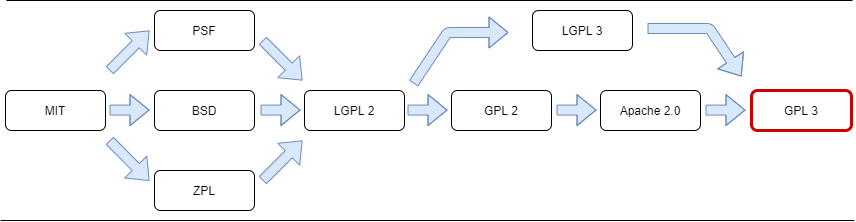
\includegraphics[width=\textwidth]{img/Diagramas/LicenseComp.png}
    \caption{Compatibilidad entre licencias. } \label{LicenseComp}
\end{figure}

El liberar el código bajo GPL3~\cite{lic:GPL3} resulta beneficioso ya que al ser de libre disposición cualquiera puede beneficiarse de éste, del mismo modo que puede mejorarlo y licenciarlo con una licencia libre compatible y poder aprovechar también dichas mejoras en futuros desarrollos. 

Por ello, para entender que permite la licencia GPL3~\cite{lic:GPL3} he confeccionado un breve resumen. Aunque la tabla~\ref{tab:GPL3} no representa la casuística completa de la licencia si nos permite tener una idea global del funcionamiento de ésta.

\footnotesize%%%%%%%%%%%  smaller font size %%%%%%%%
\begin{longtable}[c]{@{}lll@{}}
\toprule
\multicolumn{1}{c}{\textbf{Permitido}} & \multicolumn{1}{c}{\textbf{Limitaciones}} & \multicolumn{1}{c}{\textbf{Obligaciones}} \\* \midrule
\endfirsthead
%
\endhead
%
\bottomrule
\endfoot
%
\endlastfoot
%
Uso Comercial y privado. & \begin{tabular}[c]{@{}l@{}}Se prohíbe la concesión\\de sublicencias.\end{tabular} & Se debe incluir el software original. \\
El código se puede modificar. & Responsabilidad limitada. & \begin{tabular}[c]{@{}l@{}}Debe incluir los cambios en\\ el software.\end{tabular} \\
El código se puede distribuir. & No dispone de garantía. & \begin{tabular}[c]{@{}l@{}}El código debe divulgarse bajo\\una licencia compatible\\con GPL 3.0.\end{tabular} \\
\begin{tabular}[c]{@{}c@{}}Se puede otorgar garantía al \\ código con licencia.\end{tabular} &  & Debe incluir la licencia. \\* \bottomrule 
\caption{GPL3}
\label{tab:GPL3}
\end{longtable}
\normalsize Podemos ampliar la información en la página oficial de GNU~\cite{lic:GPL3}.

\subsubsection{Documentación}

Para generar la documentación se han utilizado dos licencias, la referente a~\LaTeX{} y a la aplicación Fritzing. Los diagramas electrónicos del proyecto han sigo generados con esta licencia Creative Commons by-sa~\cite{lic:CCbysa3}. La documentación del proyecto tiene la misma cobertura CC by-sa, que permite el uso comercial y distribución tanto de esta obra como derivadas de ésta siempre que se cuente con la misma licencia que regula la obra original. Podemos ver los derechos adquiridos de la obra así como las obligaciones en la página oficial~\cite{lic:CCbysa3}.

\begin{longtable}[c]{@{}lll@{}}
\toprule
\multicolumn{1}{c}{\textbf{Nombre}} & \multicolumn{1}{c}{\textbf{Licencia}} & \multicolumn{1}{c}{\textbf{Descripción}} \\* \midrule
\endfirsthead
%
\endhead
%
\bottomrule
\endfoot
%
\endlastfoot
%
\LaTeX{}~\cite{wiki:latex} & LPPL & Procesador de textos \\
Fritzing & CC by-sa & Diagramas electrónicos \\* \bottomrule \\
\caption{Dependecncias en la documentación.}
\label{tab:my-table}\\
\end{longtable}


\subsubsection{Resumen del licenciamiento del presente proyecto}
Para facilitar la búsqueda y comprensión de las licencias con que cuenta el proyecto he generado la tabla resúmen~\ref{tab:licproy} y también pueden ver las licencias en los enlaces correspondientes de GPL3~\cite{lic:GPL3} y CC-BY-SA-3.0~\cite{lic:CCbysa3}.

\begin{longtable}[c]{@{}ll@{}}
\toprule
\multicolumn{1}{c}{\textbf{Recurso}} & \multicolumn{1}{c}{\textbf{Licencia}} \\* \midrule
\endfirsthead
%
\endhead
%
\bottomrule
\endfoot
%
\endlastfoot
%
Código Fuente & GPL3 \\
Documentación & CC-BY-SA-3.0 \\
Imágenes & CC-BY-SA-3.0 \\
Vídeos & CC-BY-SA-3.0 \\* \bottomrule \\
\caption{Licencias que protegen el proyecto.}
\label{tab:licproy}\\
\end{longtable}


\begin{figure}[h]
  \begin{subfigure}
    
\includegraphics[width=0.3\textwidth]{img/Diagramas/gplv3-with-text-136x68.png}
  \end{subfigure}
  \hfill
  \begin{subfigure}
    
\includegraphics[width=0.3\textwidth]{img/Diagramas/ccbysa.png}
  \end{subfigure}
\end{figure}


\apendice{Especificación de Requisitos}
\section{Introducción}
En este punto se detallan los requisitos con que debe cumplir el proyecto y que determinarán restricciones, funcionalidades y comportamiento de éste. 

\section{Objetivos generales}
Los objetivos generales enmarcan la funcionalidad del proyecto, que se detallan a continuación:
\begin{itemize}
    \item Crear una plataforma que consiga aumentar confort, comodidad y seguridad dentro del domicilio.
    \item Generar un Sistema Domótico que nos permita automatizar parámetros de la vivienda así como poder ordenar acciones en tiempo real.
    \item Crear un Sistema Simulador de Presencia Domiciliaria de funcionamiento autónomo.
    \item Debe contar con una interfaz de comunicación multiplataforma para interactuar con el software.
\end{itemize}

\section{Catálogo de requisitos}
En este punto se desglosan los requisitos con que debe cumplir el proyecto, derivando de los anteriormente expuestos.

\subsection{\textbf{Requisitos funcionales}}

\begin{itemize}
    \item \textbf{RF-1 Obtención de datos:} El Sistema debe ser capaz de obtener datos necesarios para su correcto funcionamiento.
    \begin{itemize}
        \item \textbf{RF-1.1 Obtención de ubicación:} Debe ser capaz de determinar su ubicación geográfica.
        \item \textbf{RF-1.2 Obtención de posición solar:} Debe poder obtener información sobre la posición solar con respecto del planeta según su ubicación geográfica.
        \item \textbf{RF-1.3 Obtención de temperaturas:} Debe poder obtener información meteorológica de las próximas horas en la ubicación en la que se encuentra el Sistema.
        \item \textbf{RF-1.4 Datos bajo demanda:} El usuario debe poder solicitar la obtención de los datos bajo demanda.
    \end{itemize}

    \item \textbf{RF-2 Control de periféricos:} El Sistema debe poder controlar los periféricos que tiene conectados.
    \begin{itemize}
        \item \textbf{RF-2.1 Control automático:} El sistema debe poder controlar de forma autónoma los dispositivos conectados.
        \item \textbf{RF-2.2 Control instantáneo:} El usuario debe poder controlar los diferentes periféricos a placer.
        \item \textbf{RF-2.3 Control planificado:} El sistema debe poder planificar el control de los periféricos conectados.
        \item \textbf{RF-2.4 Parametrización:} El usuario debe poder parametrizar la automatización de los periféricos.
    \end{itemize}
    
    \item \textbf{RF-3 Información:} La información de que dispone el sistema siempre estará a disposición del usuario.
    \begin{itemize}
        \item \textbf{RF-3.1 Información de sistema:} El usuario podrá obtener información básica sobre el sistema.
        \item \textbf{RF-3.2. Información de planificación:} El usuario debe poder obtener información sobre la planificación de la automatización de los periféricos.
        \item \textbf{RF-3.3. Información parametrización:} El usuario debe poder obtener información sobre la parametrización de la automatización de los periféricos.
        \item \textbf{RF-3.4 Diagramas:} El usuario debe poder obtener un diagrama de temperaturas del día u otros días anteriores que estén archivados en la máquina a modo de registro.
    \end{itemize}
    
    \item \textbf{RF-4 Control máquina:} Se deben poder ejecutar algunas tareas básicas sobre la máquina que soporta el Sistema.
    \begin{itemize}
        \item \textbf{RF-4.1 Operaciones bajo demanda:} El usuario podrá apagar y reiniciar la máquina siempre que lo desee.
        \item \textbf{RF-4.2 Operaciones automáticas:} El sistema se reiniciará, al menos, una vez al día.
    \end{itemize}   
    
    \item \textbf{RF-5 Gestión de la máquina:} La máquina que soporta el sistema debe poder ser accesible por parte del usuario.
    \begin{itemize}
        \item \textbf{RF-5.1 Gestión local:} El usuario podrá gestionar el sistema Operativo de la máquina que soporta el Sistema de forma local.
        \item \textbf{RF-5.2 Gestión remota:} El usuario podrá gestionar el sistema Operativo de la máquina que soporta el Sistema de forma remota vía VNC.
    \end{itemize}
    
    \item \textbf{RF-6 Comunicación entre BackEnd y FrontEnd:} Debe existir un filtro en las comunicaciones.
    \begin{itemize}
        \item \textbf{RF-6.1 Selección de usuarios:} El propio usuario debe poder gestionar los usuarios que pueden interactuar con el Sistema.
        \item \textbf{RF-6.2 Rechazo de peticiones:} Los usuarios que no estén admitidos en la lista no podrán acceder a la comunicación con el Sistema.
        \item \textbf{RF-6.3 Interacción multiplataforma:} Debe poder interactuar mediante las aplicaciones móviles existentes de Telegram y desde cualquier navegador popularmente extendido como pueden ser Chrome, Edge o Firefox entre otros. 
    \end{itemize}
\end{itemize}

\subsection{\textbf{Requisitos no funcionales}}

\begin{itemize}
    \item \textbf{RNF-1 Escalabilidad:} Debe poder ampliarse fácilmente.
    \item \textbf{RNF-2 Eficiencia:} Debe minimizar la carga computacional para minimizar también el consumo energético del Sistema, además de permitir que la temperatura exterior incida en menos medida en las condiciones deseadas optimizando el consumo de recursos.
    \item \textbf{RNF-3 Rendimiento:} El sistema debe ser fluido y evitar cargas innecesarias.
    \item \textbf{RNF-4 Usabilidad:} El FrontEnd debe ser lo más usable posible, es decir, fácil de utilizar y aprender e intuitivo, y adaptado a las necesidades que pretende cubrir.
    \item \textbf{RNF-5 Disponibilidad:} El Sistema debe estar siempre en correcto funcionamiento.
    \item \textbf{RNF-6 Durabilidad:} El software debe poder funcionar correctamente durante un tiempo relativamente largo.
    \item \textbf{RNF-7 Capacidad:} Debe poder obtener la información necesaria y actuar conforme a lo que se espera de él.
    \item \textbf{RNF-8 Documentación:} Debe existir la suficiente documentación para poder implementar e interactuar con el Sistema.
    \item \textbf{RNF-9 Operabilidad:} Debe permitir manejar y controlar el Sistema según los requisitos funcionales.
    \item \textbf{RNF-10 Mantenibilidad:} Debe desarrollarse de tal manera que el mantenimiento sea lo más fácil y rápido posible.
    \item \textbf{RNF-11 Seguridad:} Todas las operaciones desde el FrontEnd deben ser seguras y estar cifradas.
    \item \textbf{RNF-12 Legibilidad:} El software debe ser fácilmente legible.
    \item \textbf{RNF-13 Extensibilidad:} El código debe ser fácilmente adaptable y reutilizable.
    \item \textbf{RNF-14 Liberación de código:} Debe disponer de un Sistema Operativo GNU y el código debe tener algún tipo de licencia GNU.
    \item \textbf{RNF-15 Respaldo documental:} Toda la instalación debe realizarse conforme a los estándares legales vigentes.
~\\~\\~\\~\\
\end{itemize}

\section{Especificación de requisitos}
La especificación de requisitos contempla los casos de uso contra nuestro código.
Además, también podemos ver el diagrama de los casos de uso, aunque lo he dividido en las figuras <<1/2>>~\ref{CDU1} y <<2/2>>~\ref{CDU2}

\begin{figure}[h]
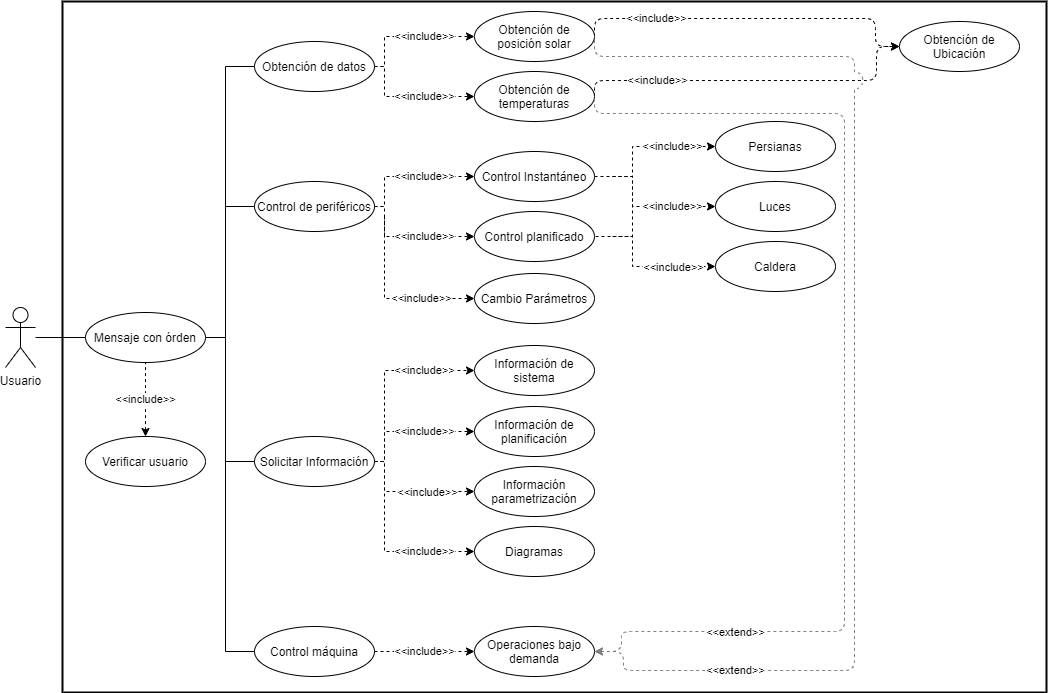
\includegraphics[width=1.15\textwidth]{img/Diagramas/CasosDeUso.png}
\caption{Casos de uso 1/2.}\label{CDU1}
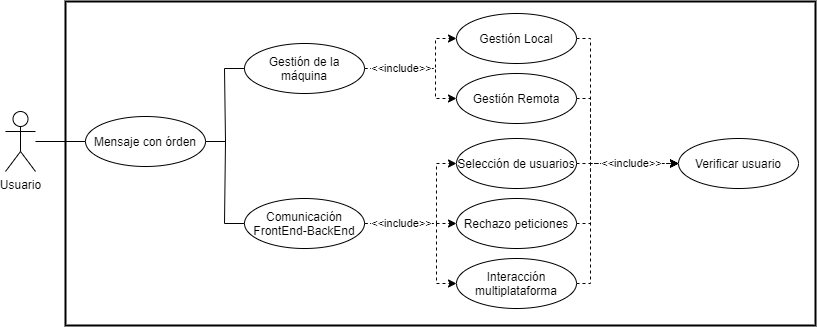
\includegraphics[width=0.85\textwidth]{img/Diagramas/CasosDeUsoBackEnd.png}
\caption{Casos de uso 2/2.}\label{CDU2}
\end{figure}

\subsection{Actores}
Los actores serán cada uno de los usuarios del Sistema que controlará el sistema desde el FrontEnd.

\footnotesize%%%%%%%%%%%  smaller font size %%%%%%%%
\begin{longtable}{>{\hspace{0pt}}m{0.182\linewidth}>{\hspace{0pt}}m{0.758\linewidth}}
\hline
\rowcolor[rgb]{0.937,0.937,0.937} \multicolumn{1}{|>{\hspace{0pt}}m{0.182\linewidth}|}{\textbf{CU-01}} & \multicolumn{1}{>{\hspace{0pt}}m{0.758\linewidth}|}{\textbf{Obtención de posición solar}} \endfirsthead 
\hline
\textbf{Versión} & 1.0 \\
\rowcolor[rgb]{0.937,0.937,0.937} \textbf{Actor} & Usuario \\
\textbf{Requisitos asociados} & RF-1, RF-1.1, RF-1.2, RF-1.3, RF-1.4 \\
\rowcolor[rgb]{0.937,0.937,0.937} \textbf{Descripción} & Permite al usuario obtener los datos necesarios para parametrizar el Sistema Domótico Inteligente. \\
\textbf{Precondición} & \begin{tabular}{@{\labelitemi\hspace{\dimexpr\labelsep+0.5\tabcolsep}}l}Al ser un proceso principalmente automático, únicamente se~\end{tabular}\par{}~ ~ requiere una línea de datos con acceso a Internet.\par\par{}\begin{tabular}{@{\labelitemi\hspace{\dimexpr\labelsep+0.5\tabcolsep}}l}En el caso de hacer la petición el usuario, también necesita~\end{tabular}\par{}~ ~ ser uno de los usuarios autorizados. \\
\rowcolor[rgb]{0.937,0.937,0.937} \textbf{Acciones} & \begin{tabular}{@{\labelitemi\hspace{\dimexpr\labelsep+0.5\tabcolsep}}>{\cellcolor[rgb]{0.937,0.937,0.937}}l}El usuario solicita la obtención inmediata de los datos~\end{tabular}\par{}necesarios para realizar la próxima programación.\par\par{}\begin{tabular}{@{\labelitemi\hspace{\dimexpr\labelsep+0.5\tabcolsep}}>{\cellcolor[rgb]{0.937,0.937,0.937}}l}El programa llama a las APIS de geolocalización,~\end{tabular}\par{}astrológicos y meteorológicos. \\
\textbf{Postcondición} & El bot lanza los scripts de recopilación de datos y almacena los datos. \\
\rowcolor[rgb]{0.937,0.937,0.937} \textbf{Excepciones} & Si no puede recopilar los datos envía mensaje al usuario. \\
\textbf{Importancia} & Alta \\\hline\\
\caption{CU-01 - Obtención de datos}\\ 
\end{longtable}


\begin{longtable}{>{\hspace{0pt}}m{0.278\linewidth}>{\hspace{0pt}}m{0.662\linewidth}}
\hline
\rowcolor[rgb]{0.937,0.937,0.937} \multicolumn{1}{|>{\hspace{0pt}}m{0.278\linewidth}|}{\textbf{CU-02}} & \multicolumn{1}{>{\hspace{0pt}}m{0.662\linewidth}|}{\textbf{Control de periféricos}} \endfirsthead 
\hline
\textbf{Versión} & 1.0 \\
\rowcolor[rgb]{0.937,0.937,0.937} \textbf{Actor} & Usuario \\
\textbf{Requisitos asociados} & RF-2, RF-2.1, RF-2.2, RF-2.3, RF-2.4 \\
\rowcolor[rgb]{0.937,0.937,0.937} \textbf{Descripción} & Permite controlar los periféricos \\
\textbf{Precondición} & \begin{tabular}{@{\labelitemi\hspace{\dimexpr\labelsep+0.5\tabcolsep}}l}Deben existir periféricos y estar configurados en el~\end{tabular}\par{}archivo al efecto.\par\par{}\begin{tabular}{@{\labelitemi\hspace{\dimexpr\labelsep+0.5\tabcolsep}}l}El usuario debe estar acreditado.\end{tabular} \\
\rowcolor[rgb]{0.937,0.937,0.937} \textbf{Acciones} & \begin{tabular}{@{\labelitemi\hspace{\dimexpr\labelsep+0.5\tabcolsep}}>{\cellcolor[rgb]{0.937,0.937,0.937}}l}El usuario puede ordenar controlar un elemento.\end{tabular} \\
\textbf{Postcondición} & El~periférico cambia de estado. \\
\rowcolor[rgb]{0.937,0.937,0.937} \textbf{Excepciones} & Si no puede realizar la acción envía mensaje al usuario. \\
\textbf{Importancia} & Media \\
\hline\\
\caption{CU-02 - Control de periféricos.}~\\~\\~\\~\\
\end{longtable}


\begin{longtable}{>{\hspace{0pt}}m{0.273\linewidth}>{\hspace{0pt}}m{0.668\linewidth}}\hline
\rowcolor[rgb]{0.937,0.937,0.937} \multicolumn{1}{|>{\hspace{0pt}}m{0.273\linewidth}|}{\textbf{CU-03}} & \multicolumn{1}{>{\hspace{0pt}}m{0.668\linewidth}|}{\textbf{Parametrización~de periféricos}} \endfirsthead 
\hline
\textbf{Versión} & 1.0 \\
\rowcolor[rgb]{0.937,0.937,0.937} \textbf{Actor} & Usuario \\
\textbf{Requisitos asociados} & RF-2, RF-2.4 \\
\rowcolor[rgb]{0.937,0.937,0.937} \textbf{Descripción} & Permite parametrizar el control automático \\
\textbf{Precondición} & \begin{tabular}{@{\labelitemi\hspace{\dimexpr\labelsep+0.5\tabcolsep}}l}Deben existir periféricos y estar configurados en el~\end{tabular}\par{}archivo al efecto.\par\par{}\begin{tabular}{@{\labelitemi\hspace{\dimexpr\labelsep+0.5\tabcolsep}}l}El usuario debe estar acreditado.\end{tabular}\par\par{}\begin{tabular}{@{\labelitemi\hspace{\dimexpr\labelsep+0.5\tabcolsep}}l}Deben introducirse los parámetros correctos.\end{tabular} \\
\rowcolor[rgb]{0.937,0.937,0.937} \textbf{Acciones} & El usuario parametriza la automatización de un periférico. \\
\textbf{Postcondición} & El~periférico cambiará de estado. \\
\rowcolor[rgb]{0.937,0.937,0.937} \textbf{Excepciones} & Si no puede realizar la acción envía mensaje al usuario. \\
\textbf{Importancia} & Alta \\
\hline
\\\caption{CU-03 - Parametrización de periféricos}
\end{longtable}

\begin{longtable}{>{\hspace{0pt}}m{0.207\linewidth}>{\hspace{0pt}}m{0.733\linewidth}}
\hline
\rowcolor[rgb]{0.937,0.937,0.937} \multicolumn{1}{|>{\hspace{0pt}}m{0.207\linewidth}|}{\textbf{CU-04}} & \multicolumn{1}{>{\hspace{0pt}}m{0.733\linewidth}|}{\textbf{Solicitar Información}} \endfirsthead 
\hline
\textbf{Versión} & 1.0 \\
\rowcolor[rgb]{0.937,0.937,0.937} \textbf{Actor} & Usuario \\
\textbf{Requisitos \mbox{asociados}} & RF-3, RF-3.1, RF-3.2, RF-3.3, RF-3.4 \\
\rowcolor[rgb]{0.937,0.937,0.937} \textbf{Descripción} & Permite obtener información del sistema, de automatización, de la parametrización. \\
\textbf{Precondición} & \begin{tabular}{@{\labelitemi\hspace{\dimexpr\labelsep+0.5\tabcolsep}}l}El usuario debe estar acreditado.\\Debe existir la información.\end{tabular} \\
\rowcolor[rgb]{0.937,0.937,0.937} \textbf{Acciones} & Lectura de información. \\
\textbf{Postcondición} & Se envía información del sistema. \\
\rowcolor[rgb]{0.937,0.937,0.937} \textbf{Excepciones} & Si no puede realizar la acción envía mensaje al usuario. \\
\textbf{Importancia} & Baja \\
\hline
\\ \caption{CU-04 Solicitar Información}\\ 
\end{longtable}

\begin{longtable}{>{\hspace{0pt}}m{0.278\linewidth}>{\hspace{0pt}}m{0.662\linewidth}}
\hline
\rowcolor[rgb]{0.937,0.937,0.937} \multicolumn{1}{|>{\hspace{0pt}}m{0.278\linewidth}|}{\textbf{CU-05}} & \multicolumn{1}{>{\hspace{0pt}}m{0.662\linewidth}|}{\textbf{Solicitar Información de sistema}} \endfirsthead 
\hline
\textbf{Versión} & 1.0 \\
\rowcolor[rgb]{0.937,0.937,0.937} \textbf{Actor} & Usuario \\
\textbf{Requisitos asociados} & RF-3, RF-3.1 \\
\rowcolor[rgb]{0.937,0.937,0.937} \textbf{Descripción} & Permite obtener información del sistema \\
\textbf{Precondición} & \begin{tabular}{@{\labelitemi\hspace{\dimexpr\labelsep+0.5\tabcolsep}}l}El usuario debe estar acreditado.\\Debe existir el diagrama.\end{tabular} \\
\rowcolor[rgb]{0.937,0.937,0.937} \textbf{Acciones} & Se envía información del sistema. \\
\textbf{Postcondición} & Se enviará la información solicitada. \\
\rowcolor[rgb]{0.937,0.937,0.937} \textbf{Excepciones} & Si no puede realizar la acción envía mensaje al usuario. \\
\textbf{Importancia} & Baja \\
\hline
\\\caption{CU-05 Solicitar Información de sistema} 
\end{longtable}

\begin{longtable}{>{\hspace{0pt}}m{0.2\linewidth}>{\hspace{0pt}}m{0.741\linewidth}}
\hline
\rowcolor[rgb]{0.937,0.937,0.937} \multicolumn{1}{|>{\hspace{0pt}}m{0.2\linewidth}|}{\textbf{CU-06}} & \multicolumn{1}{>{\hspace{0pt}}m{0.741\linewidth}|}{\textbf{Solicitar Información de planificación}} \endfirsthead 
\hline
\textbf{Versión} & 1.0 \\
\rowcolor[rgb]{0.937,0.937,0.937} \textbf{Actor} & Usuario \\
\textbf{Requisitos \mbox{asociados}} & RF-3, RF-3.1 \\
\rowcolor[rgb]{0.937,0.937,0.937} \textbf{Descripción} & Permite obtener información sobre la planificación del funcionamiento de los periféricos. \\
\textbf{Precondición} & \begin{tabular}{@{\labelitemi\hspace{\dimexpr\labelsep+0.5\tabcolsep}}l}El usuario debe estar acreditado.\\Debe existir el diagrama.\end{tabular} \\
\rowcolor[rgb]{0.937,0.937,0.937} \textbf{Acciones} & Lectura de información. \\
\textbf{Postcondición} & Se envía información del sistema \\
\rowcolor[rgb]{0.937,0.937,0.937} \textbf{Excepciones} & Si no puede realizar la acción envía mensaje al usuario. \\
\textbf{Importancia} & Baja \\
\hline
\caption{CU-06 Solicitar Información de planificación}\\ 
\end{longtable}


\begin{longtable}{>{\hspace{0pt}}m{0.19\linewidth}>{\hspace{0pt}}m{0.75\linewidth}}
\hline
\rowcolor[rgb]{0.937,0.937,0.937} \multicolumn{1}{|>{\hspace{0pt}}m{0.19\linewidth}|}{\textbf{CU-07}} & \multicolumn{1}{>{\hspace{0pt}}m{0.75\linewidth}|}{\textbf{Solicitar Información de parametrización}} \endfirsthead 
\hline
\textbf{Versión} & 1.0 \\
\rowcolor[rgb]{0.937,0.937,0.937} \textbf{Actor} & Usuario \\
\textbf{Requisitos \mbox{asociados}} & RF-3, RF-3.1 \\
\rowcolor[rgb]{0.937,0.937,0.937} \textbf{Descripción} & Permite obtener información sobre los parámetros personalizados introducidos por el usuario. \\
\textbf{Precondición} & \begin{tabular}{@{\labelitemi\hspace{\dimexpr\labelsep+0.5\tabcolsep}}l}El usuario debe estar acreditado.\\Debe existir el diagrama.\end{tabular} \\
\rowcolor[rgb]{0.937,0.937,0.937} \textbf{Acciones} & Lectura de información. \\
\textbf{Postcondición} & Se envia información de parametrización. \\
\rowcolor[rgb]{0.937,0.937,0.937} \textbf{Excepciones} & Si no puede realizar la acción envía mensaje al usuario. \\
\textbf{Importancia} & Baja \\
\hline
\caption{CU-07 Solicitar Información de parametrización}\\ 
\end{longtable}


\begin{longtable}{>{\hspace{0pt}}m{0.19\linewidth}>{\hspace{0pt}}m{0.75\linewidth}}
\hline
\rowcolor[rgb]{0.937,0.937,0.937} \multicolumn{1}{|>{\hspace{0pt}}m{0.19\linewidth}|}{\textbf{CU-08}} & \multicolumn{1}{>{\hspace{0pt}}m{0.75\linewidth}|}{\textbf{Solicitar Diagramas informativos}} \endfirsthead 
\hline
\textbf{Versión} & 1.0 \\
\rowcolor[rgb]{0.937,0.937,0.937} \textbf{Actor} & Usuario \\
\textbf{Requisitos \mbox{asociados}} & RF-3, RF-3.1 \\
\rowcolor[rgb]{0.937,0.937,0.937} \textbf{Descripción} & Permite obtener información sobre los parámetros personalizados introducidos por el usuario. \\
\textbf{Precondición} & \begin{tabular}{@{\labelitemi\hspace{\dimexpr\labelsep+0.5\tabcolsep}}l}El usuario debe estar acreditado.\\Debe existir el diagrama.\end{tabular} \\
\rowcolor[rgb]{0.937,0.937,0.937} \textbf{Acciones} & Busca el diagrama elegido. \\
\textbf{Postcondición} & Envía el diagrama. \\
\rowcolor[rgb]{0.937,0.937,0.937} \textbf{Excepciones} & Si no puede realizar la acción envía mensaje al usuario. \\
\textbf{Importancia} & Baja \\
\hline
\caption{CU-08 Solicitar Diagramas informativos}\\ 
\end{longtable}


\begin{longtable}{>{\hspace{0pt}}m{0.267\linewidth}>{\hspace{0pt}}m{0.674\linewidth}}
\hline
\rowcolor[rgb]{0.937,0.937,0.937} \multicolumn{1}{|>{\hspace{0pt}}m{0.267\linewidth}|}{\textbf{CU-09}} & \multicolumn{1}{>{\hspace{0pt}}m{0.674\linewidth}|}{\textbf{Operaciones bajo demanda}} \endfirsthead 
\hline
\textbf{Versión} & 1.0 \\
\rowcolor[rgb]{0.937,0.937,0.937} \textbf{Actor} & Usuario \\
\textbf{Requisitos asociados} & RF-4, RF-4.1 \\
\rowcolor[rgb]{0.937,0.937,0.937} \textbf{Descripción} & Permite ejecutar apagado y reinicio de la máquina a placer. \\
\textbf{Precondición} & El usuario debe estar acreditado. \\
\rowcolor[rgb]{0.937,0.937,0.937} \textbf{Acciones} & Apaga o Reinicia el Sistema. \\
\textbf{Postcondición} & La máquina ejecuta la órden enviada. \\
\rowcolor[rgb]{0.937,0.937,0.937} \textbf{Excepciones} & Si no puede realizar la acción envía mensaje al usuario. \\
\textbf{Importancia} & Baja \\
\hline
\\\caption{CU-09 Operaciones bajo demanda}\\ 
\end{longtable}

\begin{longtable}{>{\hspace{0pt}}m{0.24\linewidth}>{\hspace{0pt}}m{0.701\linewidth}}
\hline
\rowcolor[rgb]{0.937,0.937,0.937} \multicolumn{1}{|>{\hspace{0pt}}m{0.24\linewidth}|}{\textbf{CU-10}} & \multicolumn{1}{>{\hspace{0pt}}m{0.701\linewidth}|}{Gestión local de la máquina} \endfirsthead 
\hline
\textbf{Versión} & 1.0 \\
\rowcolor[rgb]{0.937,0.937,0.937} \textbf{Actor} & Usuario \\
\textbf{Requisitos \mbox{asociados}} & RF-5, RF-5.1 \\
\rowcolor[rgb]{0.937,0.937,0.937} \textbf{Descripción} & Permite administrar la máquina que soporta el sistema de forma local \\
\textbf{Precondición} & El usuario existir en el sistema. \\
\rowcolor[rgb]{0.937,0.937,0.937} \textbf{Acciones} & Administrar el sistema. \\
\textbf{Postcondición} & Si conoce las credenciales podrá administrar el sistema.  \\
\rowcolor[rgb]{0.937,0.937,0.937} \textbf{Excepciones} & Si no puede realizar la acción envía mensaje al usuario. \\
\textbf{Importancia} & Alta \\
\hline
\\\caption{CU-10 Gestión local de la máquina}\\ 
\end{longtable}

\begin{longtable}{>{\hspace{0pt}}m{0.232\linewidth}>{\hspace{0pt}}m{0.708\linewidth}}
\hline
\rowcolor[rgb]{0.937,0.937,0.937} \multicolumn{1}{|>{\hspace{0pt}}m{0.232\linewidth}|}{\textbf{CU-11}} & \multicolumn{1}{>{\hspace{0pt}}m{0.708\linewidth}|}{Gestión remota de la máquina} \endfirsthead 
\hline
\textbf{Versión} & 1.0 \\
\rowcolor[rgb]{0.937,0.937,0.937} \textbf{Actor} & Usuario \\
\textbf{Requisitos \mbox{asociados}} & RF-5, RF-5.2 \\
\rowcolor[rgb]{0.937,0.937,0.937} \textbf{Descripción} & Permite administrar la máquina que soporta el sistema de forma remota~ \\
\textbf{Precondición} & El usuario debe existir en el sistema, VNC debe estar funcionando y conocer las credenciales. \\
\rowcolor[rgb]{0.937,0.937,0.937} \textbf{Acciones} & Administrar el sistema. \\
\textbf{Postcondición} & Si conoce las credenciales podrá administrar el sistema. \\
\rowcolor[rgb]{0.937,0.937,0.937} \textbf{Excepciones} & Si no puede realizar la acción envía mensaje al usuario. \\
\textbf{Importancia} & Alta \\
\hline
\\\caption{CU-11 Gestión remota de la máquina}\\ 
\end{longtable}

\begin{longtable}{>{\hspace{0pt}}m{0.179\linewidth}>{\hspace{0pt}}m{0.762\linewidth}}
\hline
\rowcolor[rgb]{0.937,0.937,0.937} \multicolumn{1}{|>{\hspace{0pt}}m{0.179\linewidth}|}{\textbf{CU-12}} & \multicolumn{1}{>{\hspace{0pt}}m{0.762\linewidth}|}{Selección de usuarios} \endfirsthead 
\hline
\textbf{Versión} & 1.0 \\
\rowcolor[rgb]{0.937,0.937,0.937} \textbf{Actor} & Usuario \\
\textbf{Requisitos asociados} & RF-6, RF-6.1, RF-6.2 \\
\rowcolor[rgb]{0.937,0.937,0.937} \textbf{Descripción} & Se deben poder escoger los usuarios que podrán interactuar con el bot, el resto quedan descartados. \\
\textbf{Precondición} & Los usuarios seleccionados deben existir en el archivo creado para ello. \\
\rowcolor[rgb]{0.937,0.937,0.937} \textbf{Acciones} & Permite interactuar con el bot o rechaza las peticiones. \\
\textbf{Postcondición} & Si está acreditado podrá interactuar con el sistema. \\
\rowcolor[rgb]{0.937,0.937,0.937} \textbf{Excepciones} & Si no puede realizar la acción envía mensaje al usuario. \\
\textbf{Importancia} & Alta \\
\hline
\\\caption{CU-12 Selección de usuarios}\\ 
\end{longtable}


\begin{longtable}{>{\hspace{0pt}}m{0.213\linewidth}>{\hspace{0pt}}m{0.727\linewidth}}
\hline
\rowcolor[rgb]{0.937,0.937,0.937} \multicolumn{1}{|>{\hspace{0pt}}m{0.213\linewidth}|}{\textbf{CU-13}} & \multicolumn{1}{>{\hspace{0pt}}m{0.727\linewidth}|}{Interacción Multiplaforma} \endfirsthead 
\hline
\textbf{Versión} & 1.0 \\
\rowcolor[rgb]{0.937,0.937,0.937} \textbf{Actor} & Usuario \\
\textbf{Requisitos \mbox{asociados}} & RF-6, RF-6.1, RF-6.2, RF-6.3 \\
\rowcolor[rgb]{0.937,0.937,0.937} \textbf{Descripción} & Debe poder interactuar desde un usuario existente y desde cualquier plataforma. \\
\textbf{Precondición} & El usuario debe existir y estar acreditado. \\
\rowcolor[rgb]{0.937,0.937,0.937} \textbf{Acciones} & Permite interactuar con el bot o rechaza las peticiones. \\
\textbf{Postcondición} & Podrá interactuar con el sistema. \\
\rowcolor[rgb]{0.937,0.937,0.937} \textbf{Excepciones} & Si no puede realizar la acción envía mensaje al usuario. \\
\textbf{Importancia} & Alta \\
\hline
\\\caption{CU-13 Interacción Multiplataforma}\\ 
\end{longtable}



\normalsize

























\apendice{Especificación de diseño}

\section{Introducción}

\section{Diseño de datos}

\section{Diseño procedimental}

\section{Diseño arquitectónico}

\begin{comment}
    como se han repartido los archivos
\end{comment}


\apendice{Documentación técnica de programación}

\section{Introducción}
En este apartado se incluye la información técnica relacionada con el código, donde se incluye la estructura de directorios y los pasos necesarios para la obtención de los diferentes tokens.

\section{Estructura de directorios}
Para comprender la estructura de directorios debemos conocer las diferentes partes del proyecto y tener en cuenta que son completamente diferentes, aunque en este proyecto se han integrado para poder hacer uso del sistema domótico. 

El repositorio del proyecto se encuentra en la siguiente URL de GitHub:~\url{https://github.com/davidelinformatico/TFG}.

Tras accederal directorio raiz del proyecto vemos dos directorios, \textbf{credentials} y \textbf{source}. Dentro de \textbf{credentials} tenemos el archivo principal de configuración y dentro de \textbf{source} el resto de directorios del proyecto. Nada más acceder al directorio \textbf{source} podemos ver tres directorios principales:

\begin{figure}[h]
\centering
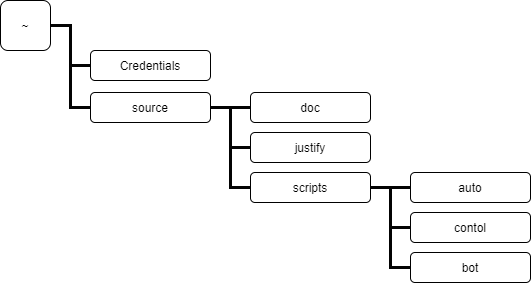
\includegraphics[width=0.9\textwidth]{img/Diagramas/directorios1.png}
\caption{Árbol de directorios del repositorio.}\label{Directorios}
\end{figure}

\begin{enumerate}
    \item El directorio~\textbf{doc} contiene la redacción del proyecto.
    \item El directorio~\textbf{justify} contiene las normativas aplicables en la instalación física.
    \item El directorio~\textbf{scripts} es el que contiene todo el código del proyecto.
\end{enumerate}

Para entender la organización del directorio que almacena el código hay que saber que el código se divide, principalmente, en tres partes, que podemos verlas en la figura~\ref{SecAcSys} son las siguientes:

\begin{itemize}
    \item La parte de toma de datos.
    \item La parte de mensajería.
    \item La parte física de nuestra instalación domótica, incluyendo la Raspberry Pi.
\end{itemize}


Por ello, dentro del directorio llamado <<scripts>> que es el que almacena nuestro código, éste se ha estructurado en tres partes:
\begin{itemize}
    \item La carpeta \textbf{auto}, que permite obtener la información de las APIs seleccionadas de Internet.
    \item La carpeta \textbf{bot}, donde almacenamos la configuración de nuestro bot.
    \item La carpeta \textbf{control}, donde almacenamos los scripts de control de la instalación domótica.
\end{itemize}

En todas ellas, los scripts, tanto de Bash como de Python llevan la cabecera específica para el tipo de código contenido en el archivo:

\begin{lstlisting}[language=python,firstnumber=0, basicstyle=\normalsize]
#!/usr/bin/env python3
\end{lstlisting}

Ésta es la cabecera para los archivos Bash:
\begin{lstlisting}[language=sh,firstnumber=0, basicstyle=\normalsize]
#!/bin/bash
\end{lstlisting}

He introducido estas cabeceras porque, sin ellas, he tenido problemas al lanzar las instrucciones desde otro script.

\subsection{Carpeta auto}
Al comienzo del proyecto esperé encontrar alguna web desde la que poder recoger la información haciendo webscraping pero tras valorarlo detenidamente en las tutorías me decanté por el uso de APIs. Uno de los motivos es que una web es más susceptible de sufrir cambios que una API que se ha predispuesto para una función específica. Finalmente, dispuse el proyecto para poder funcionar con dos APIs públicas y gratuitas para dotar a nuestro sistema domótico de autonomía.

Las siguientes fases de la parte de toma de datos, se albergan en la carpeta auto ya que es un proceso automatizado que permite al sistema obtener los datos de forma desatendida y continua.
El proceso de automatización comprende varias fases:
\begin{enumerate}
    \item La fase de~\textbf{recopilación} de datos.
    \item La fase de~\textbf{lectura} local de parámetros.
    \item El~\textbf{cocinado} de los datos.
    \item El~\textbf{grabado} de datos en el sistema local.
\end{enumerate}
La fase de~\textbf{recopilación} de datos llama a la API de~\textbf{geolocalización} y nos devuelve, entre otros, los parámetros de nuestra ubicación en formato de latitud y longitud. Posteriormente, estos datos de ubicación son necesarios para incorporarlos en la consulta de las APIs de~\textbf{meteorología} y~\textbf{astronomía} y obtener la información de la salida y puesta del sol así como la información de las temperaturas del día siguiente en dicha ubicación. Con esta recopilación de datos tenemos la base para poder determinar el comportamiento autónomo que necesitamos por lo que almacenaremos esta información en un archivo de datos.

El siguiente paso es leer las preferencias del usuario, que se almacenan en el archivo de condicionantes. Y, una vez tengamos estos datos, podemos pasar a generar el Cron para controlar de forma automática toda la instalación y generar el diagrama de temperaturas para poder enviarlo cuando se solicite. Las imágenes se almacenan dentro del directorio \texttt{./diagramas}, en formato PNG.

Estas fases se han confeccionado al final del proyecto puesto que al principio se desarrolló de forma unitaria pero surgió el problema de que, cada vez que queríamos hacer una modificación en el sistema domótico de cualquier índole, teníamos que hacer una petición nueva a las APIs y generar de nuevo un archivo Cron con los parámetros del usuario <<al vuelo>> para conseguir regenerar la automatización con los parámetros nuevos. Este sistema funcionaba correctamente pero era poco eficiente puesto que se multiplican las operaciones en función de las veces que se quiera modificar algún parámetro.
Únicamente he permitido realizar dos salidas <<al vuelo>> tras obtener los datos, estos son: el grabado de los datos recién obtenidos y la gráfica de las temperaturas conforme a dichos datos.

He tenido algunos problemas al realizar varias peticiones a las APIS ya que, por falta de permisos, no podía sobreescribir los archivos ni las imágenes. Para subsanarlo, incluí una restricción para modificar los permisos de los archivos de forma que únicamente pueden acceder el propietario y el grupo.

\subsection{Carpeta control}
La carpeta control alberga aquellos scripts bash que controlan los periféricos. Este punto únicamente me dio problemas a la hora de implantarlo desde el bot, que se subsanó con la librería os.

\subsection{Carpeta bot}
La carpeta bot contiene varios archivos, desde el archivo de control del bot hasta otros que contienen la mayoría de funcionalidades de éste. En primera instancia, se dispuso todo el código dentro del archivo de control del bot, pero por legibilidad y facilidad de mantenimiento se extrajeron las funciones.
En este punto, lo que más problemas me ha dado han sido los teclados. Como el comportamiento de los teclados es diferente entre ellos tendría que dividir las opciones del bot entre dos tipos de teclados diferentes. Finalmente, opté por no incluir estos teclados ya que no aporta funcionalidad alguna y disminuirían la legibilidad y facilidad de uso del bot. Además, para aumentar la usabilidad del bot, se ha dispuesto un menú que podemos ver al introducir el carácter <</>> además de la posibilidad de utilizar la primera letra del comando siempre que no tengamos que acompañarlo de parámetros.


\subsection{Regeneración del código al fraccionarlo por funcionalidades}

Tuve un problema en la fase de regeneración del código al fracccionarlo por funcionalidades puesto que obtenía las rutas a los archivos que necesitaba llamar de forma unitaria desde el archivo en ejecución.  Lo subsané con el siguiente código Python:
\begin{lstlisting}[language=python, firstnumber=0, basicstyle=\small, caption={Troceado de rutas}]
#!/usr/bin/env python3
#Calculamos ruta
ruta=os.getcwd().split('/')
\end{lstlisting}

Tuve que realizar un paso similar para los archivos Bash:
\begin{lstlisting}[language=sh, firstnumber=0, basicstyle=\small, caption={Obtención de rutas en Bash scripting.}]
#!/bin/bash
path=$(pwd)
\end{lstlisting}
Aunque en la segunda versión de código se utiliza desde la propia variable de sistema:

\begin{lstlisting}[language=sh, firstnumber=0, basicstyle=\small, caption={Utilización de las variables de sistema en Bash.}]
python3 ${PWD%/*}/auto/1_recabaInfo.py
python3 ${PWD%/*}/auto/3_cocinado.py
sh ${PWD%/*}/auto/4_reescribeCron.sh
\end{lstlisting}

\section{Manual del programador}
Este punto tiene como objetivo explicar los medios necesarios para continuar con el desarrollo del código así como la explicación de las partes del proyecto.
Como la parte de desarrollo se ha generado desde Raspbian OS utilizando la interfaz para desarrollo Python, <<Thonny Python IDE>>, este punto será corto ya que el propio sistema operativo dispone del software necesario.

\subsection{Requerimientos}
Para poder hacer funcionar correctamente el código se debe clonar el repositorio e instalar los <<requeriments>> que están dentro de la ruta \texttt{\textbf{/source/scripts/control/}}:
\begin{lstlisting}[language=sh, firstnumber=0, basicstyle=\normalsize, caption={Comando para instalar las librerías neceasrias.}]
pip install -r requirements
\end{lstlisting}~\\

El software necesario es:
\begin{itemize}
    \item pyTelegramBotAPI
    \item python-telegram-bot
    \item pycurl
    \item urllib3
    \item simplejson
    \item datetime
    \item requests
    \item datetime
    \item pandas
    \item matplotlib
\end{itemize}

También hay que generar el archivo de configuración al mismo nivel que nuestro directorio raíz, dentro de un directorio llamado <<\textbf{credentials}>>, llamado \texttt{config2.bot}, de forma que quede como en la imagen~\ref{Directorios}. La información que debe contener el archivo es la que figura en el código del listing~\ref{Config2.bot}, incluyendo los tokens correspondientes y los elementos a controlar.
En las <<releases>> ya se incorpora el directorio y una plantilla para rellenar el archivo \texttt{config2.bot} correctamente.

\subsection{Archivos}
Dentro del directorio \texttt{auto} encontramos:
\begin{itemize}
    \item \texttt{~/source/scripts/auto/1\_recabaInfo.py}: Obtiene la información necesaria de las APIS.
    \item \texttt{~/source/scripts/auto/2\_condicionantes.py}: Contiene preferencias de usuario.
    \item \texttt{~/source/scripts/auto/3\_cocinado.py}: Genera el archivo preliminar del Cron para controlar las instalaciones.
    \item \texttt{~/source/scripts/auto/4\_reescribeCron.sh}: Reescribe el archivo de configuración del servicio Cron y lo reinicia.
    \item \texttt{~/source/scripts/auto/cabecera.txt}: Contiene la cabecera que utilizamos para incluirla en Cron.
    \item \texttt{~/source/scripts/auto/CronPruebas}: Contiene el texto que se volcará al archivo de configuración de Cron.
    \item \texttt{~/source/scripts/auto/InfoRecabada}: Contiene la información que se ha obtenido de las APIs.
    \item \texttt{~/source/scripts/auto/LanzaTodoElProceso.sh}: Lanza los 4 primeros scripts de forma desatendida.
    \item \texttt{~/source/scripts/auto/log.cron}: Contiene información a consultar por el bot.
    \item \texttt{~/source/scripts/auto/obtencionDatos.py}: Nos permite leer el archivo ~/credentials.config2.bot y obtiene las rutas que utilizaremos.
\end{itemize}

Dentro del directorio \texttt{bot} encontramos:
\begin{itemize}
    \item \texttt{~/source/scripts/bot/bot.py}: Contiene el archivo de configuración del bot.
    \item \texttt{~/source/scripts/bot/datos.py}: Obtiene las horas de amanecer, anochecer, encendido de luces y subida de persianas por la mañana y los envía al usuario que lo solicita.
    \item \texttt{~/source/scripts/bot/diagramaTemperaturas.py}: Envía la última imagen generada por el sistema u otra que especifique el usuario.
    \item \texttt{~/source/scripts/bot/generador.py}: Lanza todo el proceso automático desde ./auto/LanzaTodoElProceso.sh.
    \item \texttt{~/source/scripts/bot/horaSubida.py}: Envía la hora a la que se subirán las persianas por la mañana y permite cambiarla si el usuario especifica otra hora siempre que ésta sea después de la hora de amanecer.
    \item \texttt{~/source/scripts/bot/info.py}: Nos muestra información de la máquina Raspberry Pi que soporta el Sistema.
    \item \texttt{~/source/scripts/bot/obtencionDatos.py}: Nos permite leer el archivo ~/credentials.config2.bot y obtiene las rutas que utilizaremos.
    \item \texttt{~/source/scripts/bot/subirPararBajar.py}: Nos permite controlar el movimiento de las persianas si existen en el archivo de configuración.
    \item \texttt{~/source/scripts/bot/temperaturaCalefaccion.py}: Envía la temperatura a la que queremos que se encienda la caldera y nos permite modificarla.
    \item \texttt{~/source/scripts/bot/temperaturasManana.py}: Envía la relación de temperaturas por horas en la ubicación de la máquina.
\end{itemize}

Dentro del directorio \texttt{control} encontramos:
\begin{itemize}
    \item \texttt{~/source/scripts/control/EncenderCaldera.sh}: Enciende la caldera.
    \item \texttt{~/source/scripts/control/ApagarCaldera.sh}: Apaga la caldera.
    \item \texttt{~/source/scripts/control/EstadoGPIO.sh}: Permite conocer el estado de los GPIO en ese instante de tiempo.
    \item \texttt{~/source/scripts/control/Bajar.sh}: Baja todas las persianas.
    \item \texttt{~/source/scripts/control/EstadoGPIO.sh}: Inhabilita los GPIO seleccionados.
    \item \texttt{~/source/scripts/control/LucesOff.sh}: Apaga las luces.
    \item \texttt{~/source/scripts/control/LucesOn.sh}: Enciende las luces.
    \item \texttt{~/source/scripts/control/Prueba\_General.sh}: Permite hacer una prueba de las persianas conectadas.
    \item \texttt{~/source/scripts/control/Reinicia\_Servicio\_Cron.sh}: Reinicia el servicio Cron.
    \item \texttt{~/source/scripts/control/subir.sh}: Sube todas las persianas.
    
\end{itemize}


\subsection{Configuración del bot como servicio}
El bot se puede lanzar como si fuera un script más pero en este caso es necesario incorporarlo como servicio. Esta decisión tiene beneficios, como la posibilidad de que se inicie con el sistema o que podamos lanzarlo o pararlo desde cualquier ubicación del SO sin tener que recordar la ubicación con la sentencia al efecto de <<\texttt{sudo service bot start/stop}>>. Pero, una vez que el demonio está corriendo, tenemos que tener en cuenta de que ya está levantada la instancia del bot, por lo que tendremos que detenerla a la hora de hacer algún tipo de modificación así como recordar que debemos levantarlo una vez terminemos. Los pasos a seguir están en un archivo dentro de \textbf{\textasciitilde/source/scripts/auto/}.

\section{Compilación, instalación y ejecución del proyecto}
Para realizar modificaciones en el código únicamente hay que seguir los siguientes pasos:
\begin{enumerate}
    \item Descargar la última release que exista en el repositorio de GitHub en el formato que se prefiera:~\url{https://github.com/davidelinformatico/TFG/releases}
    \item Para extraer del archivo .tar utilizar: 
    \begin{lstlisting}[language=sh, firstnumber=0, basicstyle=\normalsize, caption={Comando para extraer archivos .tar.}] 
tar -xvf SistemaDomoticoInteligente\_v1.3.tar \end{lstlisting}
        
    \item Para extraer del archivo .tar.gz utilizar:
    \begin{lstlisting}[language=sh, firstnumber=0, basicstyle=\normalsize, caption={Comando para extraer archivos .tar.gz}] 
tar xzvf SistemaDomoticoInteligente\_v1.3.tar.gz \end{lstlisting}
\end{enumerate}
En este punto ya tendremos todos los archivos extraídos y podremos editarlos. Recordar que para completar el software hay que instalar el software especificado en el archivo \texttt{requeriments} que se realiza de forma automática al correr el archivo setup contenido en \textbf{\textasciitilde/source/scripts/auto/}. 

Hay que tener en cuenta que en este punto no existen los archivos esperados de control de periféricos, en el directorio \textbf{control} porque se generan a medida del sistema que se configure el sistema tras completar el archivo \texttt{config2.bot} por lo que también se puede modificar la creación de estos achivos.

No hace falta un software específico para poder modificar el código ya que podemos utilizar los propios de la Raspberry Pi o algún editor sencillo como Nano según nuestras preferencias.

Si el objetivo es correr el software correctamente hay que recordar que es indispensable que el archivo config2.bot esté completo y que se lance el setup contenido en \textbf{\textasciitilde/source/scripts/auto/}.

Finalmente, el proyecto puede lanzarse corriendo el archivo de configuración del bot:~\texttt{bot.py} desde un terminal sh, aunque si se precisa también se pueden lanzar los scripts del directorio~\textbf{auto} o~\textbf{control} por separado ya que, aunque funciona todo como un conjunto, podemos probarlos de forma unitaria.


\section{Calidad del código}
Para comprobar la calidad del código se ha utilizado un servicio externo llamado SonarCloud, que está vinculado a GitHub de forma que calcula los errores en el código pudiendo mejorarlo.
Podemos acceder a las estadísticas de SonarCloud con este enlace:~\url{https://sonarcloud.io/dashboard?id=davidelinformatico_TFG}.


\section{Pruebas del sistema}
Como el proyecto no cuenta con testigos de cambios de estado de los periféricos es imposible realizar pruebas en este punto y lo mismo sucede con la parte de domótica automatizada, es imposible determinar si un código realiza correctamente una acción física ya que aunque el código funcione correctamente puede que no se esté llevando a cabo correctamente la acción.

Por otro lado, las pruebas sobre la parte del proyecto que se comunica con las APIs y procesa la información se ha realizado de forma manual ya que únicamente son dos archivos y son relativamente cortos. 


No obstante, las pruebas que se han realizado son las que aparecen en las tablas~\ref{CP-1} -~\ref{CP200}:

\begin{longtable}{>{\hspace{0pt}}m{0.25\linewidth}>{\hspace{0pt}}m{0.764\linewidth}}
\label{CP-1}
\caption{CP-1 Existencia de datos en archivo de configuración}\\ 
\hline
\rowcolor[rgb]{0.937,0.937,0.937} \multicolumn{1}{|>{\hspace{0pt}}m{0.25\linewidth}|}{\textbf{CP-1}} & \multicolumn{1}{>{\hspace{0pt}}m{0.764\linewidth}|}{Existencia de datos en archivo de configuración} \endfirsthead 
\hline
\textbf{Versión} & 1.3 \\
\rowcolor[rgb]{0.937,0.937,0.937} \textbf{\mbox{Descripción}} & Si existen datos en el archivo de configuración,el bot inicia sin errores, ya que dispone de los parámetros de \mbox{configuración}. \\
\textbf{\mbox{Precondición}} & \texttt{Config2.bot} debe contener los datos necesarios. \\
\rowcolor[rgb]{0.937,0.937,0.937} \textbf{Acciones} & Permite ejecutar el bot sin errores. \\
\textbf{\mbox{Postcondición}} & El bot envía un mensaje de inicio a todos los usuarios. \\
\rowcolor[rgb]{0.937,0.937,0.937} \textbf{\mbox{Excepciones}} & Si el archivo \texttt{config2.bot} el sistema dará error. \\
\textbf{\mbox{Importancia}} & Crítica. \\
\hline
\end{longtable}


\begin{longtable}{>{\hspace{0pt}}m{0.25\linewidth}>{\hspace{0pt}}m{0.764\linewidth}}
\caption{CP-2 Se muestra el comando de ayuda}\\ 
\hline
\rowcolor[rgb]{0.937,0.937,0.937} \multicolumn{1}{|>{\hspace{0pt}}m{0.25\linewidth}|}{\textbf{CP-2}} & \multicolumn{1}{>{\hspace{0pt}}m{0.764\linewidth}|}{Se muestra el comando de ayuda} \endfirsthead 
\hline
\textbf{Versión} & 1.3 \\
\rowcolor[rgb]{0.937,0.937,0.937} \textbf{Descripción} & Se ha configurado el comando de ayuda y la envía~\par{}cuando es necesario. \\
\textbf{Precondición} & El bot debe haber iniciado correctamente. \\
\rowcolor[rgb]{0.937,0.937,0.937} \textbf{Acciones} & Solicitamos ayuda con '\texttt{/ayuda}' . \\
\textbf{Postcondición} & El bot envía un mensaje con las opciones disponibles. \\
\rowcolor[rgb]{0.937,0.937,0.937} \textbf{Excepciones} &  \\
\textbf{Importancia} & Baja. \\
\hline~\\~\\~\\~\\~\\~\\ % para que no corte la tabla
\end{longtable}


\begin{longtable}{>{\hspace{0pt}}m{0.25\linewidth}>{\hspace{0pt}}m{0.764\linewidth}}
\caption{CP-3 Movimiento de las persianas}\\ 
\hline
\rowcolor[rgb]{0.937,0.937,0.937} \multicolumn{1}{|>{\hspace{0pt}}m{0.25\linewidth}|}{\textbf{CP-3}} & \multicolumn{1}{>{\hspace{0pt}}m{0.764\linewidth}|}{Movimiento de las persianas} \endfirsthead 
\hline
\textbf{Versión} & 1.3 \\
\rowcolor[rgb]{0.937,0.937,0.937} \textbf{Descripción} & Las persianas se mueven bajo demanda. \\
\textbf{Precondición} & El bot debe haber iniciado correctamente,\par{}obteniendo los parámetros de configuración del\par{}archivo \texttt{config2.bot}. \\
\rowcolor[rgb]{0.937,0.937,0.937} \textbf{Acciones} & Comando '\texttt{/subir}' '\texttt{estancia}' \texttt{tiempo} y~'\texttt{/bajar}' '\texttt{estancia}' \texttt{tiempo}. Por ejemplo:\par{} \texttt{/subir Cocina 3}\par{}\texttt{/bajar Dormitorio 4} \\
\textbf{Postcondición} & Se observa que la persiana de la cocina sube 3 segundos y\par{}que la persiana del dormitorio baja 4 segundos. \\
\rowcolor[rgb]{0.937,0.937,0.937} \textbf{Notas} & Este caso de pruebas hay que realizarlo con todas las~\par{}persianas, tanto en modo subida como en modo bajada. \\
\textbf{Importancia} & Media. \\
\hline
\end{longtable}

\begin{longtable}{>{\hspace{0pt}}m{0.25\linewidth}>{\hspace{0pt}}m{0.764\linewidth}}
\caption{CP-4 Envío de tabla de temperaturas}\\ 
\hline
\rowcolor[rgb]{0.937,0.937,0.937} \multicolumn{1}{|>{\hspace{0pt}}m{0.25\linewidth}|}{\textbf{CP-4}} & \multicolumn{1}{>{\hspace{0pt}}m{0.764\linewidth}|}{Envío de tabla de temperaturas} \endfirsthead 
\hline
\textbf{Versión} & 1.3 \\
\rowcolor[rgb]{0.937,0.937,0.937} \textbf{Descripción} & Se envía una tabla informativa con las temperaturas del díasiguiente por horas. Se incluyen la hora de subida de las persianas y la hora de encendido de luces y la posterior bajada de persianas y apagado de luces. \\
\textbf{Precondición} & El bot debe haber iniciado correctamente, obteniendo los parámetros de configuración del archivo \texttt{config2.bot}.~\par{}Deben existir datos en el archivo de consulta \texttt{log.bot}. \\
\rowcolor[rgb]{0.937,0.937,0.937} \textbf{Acciones} & Enviamos el comando \texttt{/temp} \\
\textbf{Postcondición} & Envía la tabla solicitada en formato HTML, con iconos. \\
\rowcolor[rgb]{0.937,0.937,0.937} \textbf{Excepción} & Si los archivos no tienen datos o no existen no se envía nada. \\
\textbf{Importancia} & Baja. \\
\hline
\end{longtable}~\\~\\~\\~\\

\begin{longtable}{>{\hspace{0pt}}m{0.25\linewidth}>{\hspace{0pt}}m{0.764\linewidth}}
\caption{CP-5 Diagrama de temperaturas}\\ 
\hline
\rowcolor[rgb]{0.937,0.937,0.937} \multicolumn{1}{|>{\hspace{0pt}}m{0.25\linewidth}|}{\textbf{CP-5}} & \multicolumn{1}{>{\hspace{0pt}}m{0.764\linewidth}|}{Diagrama de temperaturas} \endfirsthead 
\hline
\textbf{Versión} & 1.3 \\
\rowcolor[rgb]{0.937,0.937,0.937} \textbf{Descripción} & Se envía una imagen generada con las temperaturas del\par{}día siguiente. \\
\textbf{Precondición} & El bot debe haber iniciado correctamente, obteniendo los parámetros de configuración del archivo \texttt{config2.bot}. Debe existir alguna imagen \\
\rowcolor[rgb]{0.937,0.937,0.937} \textbf{Acciones} & Enviamos el comando \texttt{/d} o \texttt{/d} seguido de un nombre de imagen. \\
\textbf{Postcondición} & Envía la imagen solicitada o predeterminada. \\
\rowcolor[rgb]{0.937,0.937,0.937} \textbf{Excepción} & Si no existen los datos no hace nada. \\
\textbf{Importancia} & Baja. \\
\hline
\end{longtable}


\begin{longtable}{>{\hspace{0pt}}m{0.25\linewidth}>{\hspace{0pt}}m{0.764\linewidth}}
\caption{CP-6 Temperatura de la calefacción}\\ 
\hline
\rowcolor[rgb]{0.937,0.937,0.937} \multicolumn{1}{|>{\hspace{0pt}}m{0.25\linewidth}|}{\textbf{CP-6}} & \multicolumn{1}{>{\hspace{0pt}}m{0.764\linewidth}|}{Temperatura de la calefacción} \endfirsthead 
\hline
\textbf{Versión} & 1.3 \\
\rowcolor[rgb]{0.937,0.937,0.937} \textbf{Descripción} & Informa de la temperatura a la que se enciende la caldera, y también, nos permite modificarla. \\
\textbf{Precondición} & El bot debe haber iniciado correctamente, obteniendo los parámetros de configuración del archivo \texttt{config2.bot}. Debe haber información en el archivo \texttt{2\_condicionantes}. \\
\rowcolor[rgb]{0.937,0.937,0.937} \textbf{Acciones} & Enviamos el comando \texttt{/tempcal}, o \texttt{/tempcal} seguido \par{}de una temperatura. \\
\textbf{Postcondición} & Si se solicita cambia la temperatura y siempre envía la\par{}información sobre la temperatura a la que arranca la caldera. \\
\rowcolor[rgb]{0.937,0.937,0.937} \textbf{Excepción} & Si no existen los datos no envía la temperatura.\par{}Si se introduce otra cosa envía mensaje de error. \\
\textbf{Importancia} & Baja. \\
\hline~\\~\\~\\~\\~\\~\\~\\~\\~\\ % para que no corte la tabla
\end{longtable}

\begin{longtable}{>{\hspace{0pt}}m{0.25\linewidth}>{\hspace{0pt}}m{0.764\linewidth}}
\caption{CP-7 Información de acciones}\\ 
\hline
\rowcolor[rgb]{0.937,0.937,0.937} \multicolumn{1}{|>{\hspace{0pt}}m{0.25\linewidth}|}{\textbf{CP-7}} & \multicolumn{1}{>{\hspace{0pt}}m{0.764\linewidth}|}{Información de acciones} \endfirsthead 
\hline
\textbf{Versión} & 1.3 \\
\rowcolor[rgb]{0.937,0.937,0.937} \textbf{Descripción} & Informa de las horas de interacción con los periféricos. \\
\textbf{Precondición} & El bot debe haber iniciado correctamente, obteniendo los parámetros de configuración del archivo \texttt{config2.bot}.~\par{}Debe existir información en el archivo \texttt{log.cron}. \\
\rowcolor[rgb]{0.937,0.937,0.937} \textbf{Acciones} & Enviamos el comando \texttt{/datos}, \texttt{d} o \texttt{D}. \\
\textbf{Postcondición} & Envía la información solicitada. \\
\rowcolor[rgb]{0.937,0.937,0.937} \textbf{Excepción} & Si no existen los datos no envía la información \\
\textbf{Importancia} & Baja. \\
\hline
\end{longtable}


\begin{longtable}{>{\hspace{0pt}}m{0.25\linewidth}>{\hspace{0pt}}m{0.764\linewidth}}
\caption{CP-8 Hora de subida de las persianas}\\ 
\hline
\rowcolor[rgb]{0.937,0.937,0.937} \multicolumn{1}{|>{\hspace{0pt}}m{0.25\linewidth}|}{\textbf{CP-8}} & \multicolumn{1}{>{\hspace{0pt}}m{0.764\linewidth}|}{Hora de subida de las persianas} \endfirsthead 
\hline
\textbf{Versión} & 1.3 \\
\rowcolor[rgb]{0.937,0.937,0.937} \textbf{Descripción} & Informa de la hora de subida de las persianas y\par{}también permite modificarla. \\
\textbf{Precondición} & El bot debe haber iniciado correctamente, obteniendo los parámetros de configuración del archivo \texttt{config2.bot}.~\par{}Debe existir información en el archivo \texttt{2\_condicionantes} \\
\rowcolor[rgb]{0.937,0.937,0.937} \textbf{Acciones} & Enviamos el comando \texttt{/hora} o \texttt{/hora} seguido de una hora. \\
\textbf{Postcondición} & Envía o modifica la información solicitada. \\
\rowcolor[rgb]{0.937,0.937,0.937} \textbf{Excepción} & Si el formato no es el correcto envía mensaje de error.\par{}Si no existe la información no envía hora. \\
\textbf{Importancia} & Baja. \\
\hline~\\~\\~\\~\\~\\~\\~\\~\\~\\~\\~\\~\\ % para que no corte la tabla
\end{longtable}

\begin{longtable}{>{\hspace{0pt}}m{0.25\linewidth}>{\hspace{0pt}}m{0.764\linewidth}}
\caption{CP-9 Obtención de datos bajo demanda}\\ 
\hline
\rowcolor[rgb]{0.937,0.937,0.937} \multicolumn{1}{|>{\hspace{0pt}}m{0.25\linewidth}|}{\textbf{CP-9}} & \multicolumn{1}{>{\hspace{0pt}}m{0.764\linewidth}|}{Obtención de datos bajo demanda} \endfirsthead 
\hline
\textbf{Versión} & 1.3 \\
\rowcolor[rgb]{0.937,0.937,0.937} \textbf{Descripción} & Obtiene los datos de las APIs \\
\textbf{Precondición} & El bot debe haber iniciado correctamente, obteniendo los parámetros de configuración del archivo \texttt{config2.bot} además de los token de las APIs.\par{}Debemos tener salida a Internet. \\
\rowcolor[rgb]{0.937,0.937,0.937} \textbf{Acciones} & Enviamos el comando \texttt{/generar}. \\
\textbf{Postcondición} & Solicita la información y genera los archivos \texttt{log.cron}, \texttt{InfoRecabada}, \texttt{CronPruebas} y la implanta en \texttt{Cron}.\par{}Envía mensaje de confirmación. \\
\rowcolor[rgb]{0.937,0.937,0.937} \textbf{Excepción} & Si no hay datos en 2\_condicionantes escribe blancos. \\
\textbf{Importancia} & Alta. \\
\hline
\end{longtable}

\begin{longtable}{>{\hspace{0pt}}m{0.25\linewidth}>{\hspace{0pt}}m{0.764\linewidth}}
\caption{CP-10 Información del sistema}\\ 
\hline
\rowcolor[rgb]{0.937,0.937,0.937} \multicolumn{1}{|>{\hspace{0pt}}m{0.25\linewidth}|}{\textbf{CP-10}} & \multicolumn{1}{>{\hspace{0pt}}m{0.764\linewidth}|}{Información del sistema} \endfirsthead 
\hline
\textbf{Versión} & 1.3 \\
\rowcolor[rgb]{0.937,0.937,0.937} \textbf{Descripción} & Envía información de la máquina. \\
\textbf{Precondición} & El bot debe haber iniciado correctamente, obteniendo los parámetros de configuración del archivo \texttt{config2.bot} además de los token de las APIs. \\
\rowcolor[rgb]{0.937,0.937,0.937} \textbf{Acciones} & Enviamos el comando \texttt{/info}, \texttt{i} o \texttt{I} \\
\textbf{Postcondición} & Envía mensaje de con la información de Sistema. \\
\rowcolor[rgb]{0.937,0.937,0.937} \textbf{Excepción} &  \\
\textbf{Importancia} & Baja. \\
\hline
\end{longtable}



\begin{longtable}{>{\hspace{0pt}}m{0.25\linewidth}>{\hspace{0pt}}m{0.764\linewidth}}
\caption{CP-11 Apagado y Reinicio}\\ 
\hline
\rowcolor[rgb]{0.937,0.937,0.937} \multicolumn{1}{|>{\hspace{0pt}}m{0.25\linewidth}|}{\textbf{CP-11}} & \multicolumn{1}{>{\hspace{0pt}}m{0.764\linewidth}|}{Apagado y Reinicio} \endfirsthead 
\hline
\textbf{Versión} & 1.3 \\
\rowcolor[rgb]{0.937,0.937,0.937} \textbf{Descripción} & Apaga o reinicia la máquina \\
\textbf{Precondición} & El bot debe haber iniciado correctamente, obteniendo los parámetros de configuración del archivo \texttt{config2.bot}. \\
\rowcolor[rgb]{0.937,0.937,0.937} \textbf{Acciones} & Enviamos el comando \texttt{/apagar} o \texttt{/reiniciar}. \\
\textbf{Postcondición} & El comando \texttt{/reiniciar}, reinicia la máquina y al volver a iniciar veremos el mensaje de inicio.\par{}El comando \texttt{/apagar}, apaga la máquina.\\
\rowcolor[rgb]{0.937,0.937,0.937}
\textbf{Importancia} & Baja. \\
\hline
\end{longtable}



\begin{longtable}{>{\hspace{0pt}}m{0.25\linewidth}>{\hspace{0pt}}m{0.764\linewidth}}
\caption{CP-100 Recabado de información}\\ 
\hline
\rowcolor[rgb]{0.937,0.937,0.937} \multicolumn{1}{|>{\hspace{0pt}}m{0.25\linewidth}|}{\textbf{CP-100}} & \multicolumn{1}{>{\hspace{0pt}}m{0.764\linewidth}|}{Recabado de información} \endfirsthead 
\hline
\textbf{Versión} & 1.3 \\
\rowcolor[rgb]{0.937,0.937,0.937} \textbf{Descripción} & Llama a las APIs y obtiene la información \\
\textbf{Precondición} & El bot debe haber iniciado correctamente, obteniendo los parámetros de configuración del archivo \texttt{config2.bot}. Se debe tener línea de datos con salida a Internet. \\
\rowcolor[rgb]{0.937,0.937,0.937} \textbf{Acciones} & Lanzamos el script \texttt{python3 1\_recabaInfo.py} \\
\textbf{Postcondición} & Si consigue la información escribe el archivo \texttt{InfoRecabada}. \\
\rowcolor[rgb]{0.937,0.937,0.937} \textbf{Excepción} & Si hay excepción informa de el error \\
\textbf{Importancia} & Alta \\
\hline
\end{longtable}

\begin{longtable}{>{\hspace{0pt}}m{0.25\linewidth}>{\hspace{0pt}}m{0.764\linewidth}}
\caption{CP-101 Procesado de la información}\\ 
\hline
\rowcolor[rgb]{0.937,0.937,0.937} \multicolumn{1}{|>{\hspace{0pt}}m{0.25\linewidth}|}{\textbf{CP-101}} & \multicolumn{1}{>{\hspace{0pt}}m{0.764\linewidth}|}{Procesado de información} \endfirsthead 
\hline
\textbf{Versión} & 1.3 \\
\rowcolor[rgb]{0.937,0.937,0.937} \textbf{Descripción} & Lee el archivo \texttt{InfoRecabada} y genera el diagrama y los archivos de \texttt{CronPruebas} y \texttt{log.cron}. \\
\textbf{Precondición} & El bot debe haber iniciado correctamente, obteniendo los parámetros de configuración del archivo \texttt{config2.bot}.~\par{}Deben existir los datos. \\
\rowcolor[rgb]{0.937,0.937,0.937} \textbf{Acciones} & Lanzamos el script \texttt{python3 3\_cocinado.py} \\
\textbf{Postcondición} & Genera el diagrama y los archivos \texttt{CronPruebas} y \texttt{log.cron} \\
\rowcolor[rgb]{0.937,0.937,0.937} \textbf{Excepción} & Si hay excepción informa de el error \\
\textbf{Importancia} & Alta \\
\hline
\end{longtable}~\\~\\~\\~\\~\\~\\~\\~\\ % para que no corte la tabla


\begin{longtable}{>{\hspace{0pt}}m{0.25\linewidth}>{\hspace{0pt}}m{0.764\linewidth}}
\caption{CP-102 Configuración de Cron}\\ 
\hline
\rowcolor[rgb]{0.937,0.937,0.937} \multicolumn{1}{|>{\hspace{0pt}}m{0.25\linewidth}|}{\textbf{CP-102}} & \multicolumn{1}{>{\hspace{0pt}}m{0.764\linewidth}|}{Configuración de Cron} \endfirsthead 
\hline
\textbf{Versión} & 1.3 \\
\rowcolor[rgb]{0.937,0.937,0.937} \textbf{Descripción} & Lee el archivo \texttt{CronPruebas}, lo vuelca a \texttt{Cron} y reinicia los servicios de la máquina. \\
\textbf{Precondición} & El bot debe haber iniciado correctamente, obteniendo los parámetros de configuración del archivo \texttt{config2.bot}. Debe existir el archivo \texttt{CronPruebas}. \\
\rowcolor[rgb]{0.937,0.937,0.937} \textbf{Acciones} & Lanzamos el script \texttt{sh 4\_reescribeCron.sh}. \\
\textbf{Postcondición} & Vuelca el contenido del archivo al archivo de configuración del programador de tareas del sistema, \texttt{Cron}. Además, reinicia los servicios.\\
\rowcolor[rgb]{0.937,0.937,0.937} \textbf{Excepción} & Si el archivo \texttt{CronPruebas} está vacío, al volcarlo a \texttt{Cron},\par{}éste también lo estará. \\
\textbf{Importancia} & Alta \\
\hline
\end{longtable}

\begin{longtable}{>{\hspace{0pt}}m{0.25\linewidth}>{\hspace{0pt}}m{0.764\linewidth}}
\label{CP200}
\caption{CP-200 Cambio de estado de periféricos}\\ 
\hline
\rowcolor[rgb]{0.937,0.937,0.937} \multicolumn{1}{|>{\hspace{0pt}}m{0.25\linewidth}|}{\textbf{CP-200}} & \multicolumn{1}{>{\hspace{0pt}}m{0.764\linewidth}|}{Cambio de estado de periféricos} \endfirsthead 
\hline
\textbf{Versión} & 1.3 \\
\rowcolor[rgb]{0.937,0.937,0.937} \textbf{Descripción} & Comprobamos que los periféricos se moverán como esperamos cuando lo hagan de forma automática. \\
\textbf{Precondición} & El bot debe haber iniciado correctamente, obteniendo los parámetros de configuración del archivo \texttt{config2.bot}.~\par{}Deben existir los scripts dentro del directorio \texttt{control}. \\
\rowcolor[rgb]{0.937,0.937,0.937} \textbf{Acciones} & Lanzamos cada uno de los scripts con el comando \texttt{sh}. \\
\textbf{Postcondición} & Cambia de estado los periféricos: Sube todas las persianas, baja todas las persianas, enciende las luces, apaga las luces y enciende y apaga la caldera. \\
\rowcolor[rgb]{0.937,0.937,0.937} \textbf{Excepción} & Si no están bien conectadas las líneas de los periféricos no funcionarán correctamente. \\
\textbf{Importancia} & Alta \\
\hline
\end{longtable}










\apendice{Documentación de usuario}

\section{Introducción}

\section{Requisitos de usuarios}

\section{Instalación}

\section{Manual del usuario}





\bibliography{bibliografiaAnexos}
\bibliographystyle{plain}

\end{document}